\section{Bin Migration Effects}

        \iffalse
    t1 mean purity:  0.5779366649713987
    t1 mean efficiency:  0.6042514773951323
    t2 mean purity:  0.7249045469386235
    t2 mean efficiency:  0.7344406993707698
    t1 rad mean purity:  0.5959652676783339
    t1 rad mean efficiency:  0.6213147478696212
    t2 rad mean purity:  0.7423936456812074
    t2 rad mean efficiency:  0.7511469995793438
    \fi 
    
    
    Mean bin purity is 58\%, mean efficiency is 60\%. 

    Wrapped phi variable for binning
    We say that it is close to 3x3x3x3 kernel for nearest neighbors
    INSERT PLOT HIGHLIGHTING NEAREST NEIGHBORS
    It is a reasonable approximation
    
    
    Finite bin and bin volume effects discussed in chapter 4. Here: migration. 
    
    So far, we have discussed measuring differential \xsecs assuming a framework that we detect an event in the same four-dimensional bin that it truly lies in. For example,


    
    \begin{figure}[H]
        \centering
        \subfloat[xb vs q2]{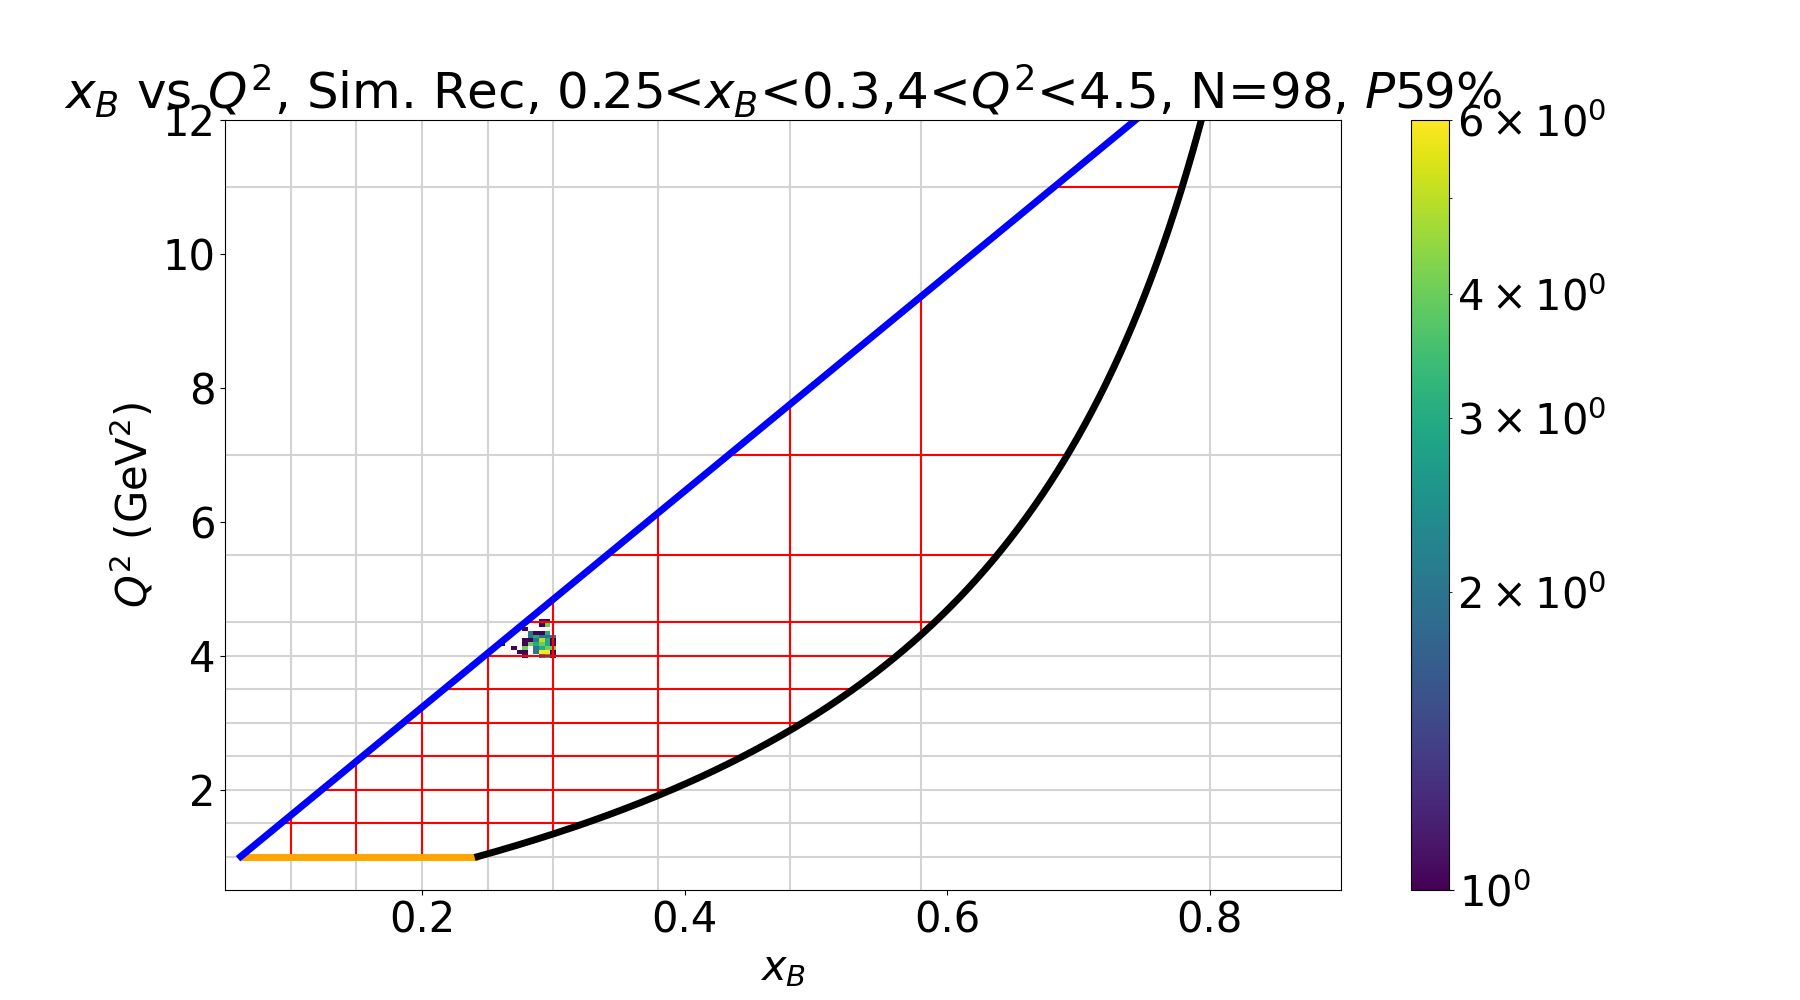
\includegraphics[trim={0 0 10cm 3.5cm},clip,width=0.52\textwidth]{Chapters/Ch5-Further/0_IBU/pics/migration_example/x_B_vs_Q2,_Sim_Rec,_025x_B03,4Q245,_N=98,_P59.png}}
        \hfill
        \subfloat[phi vs t]{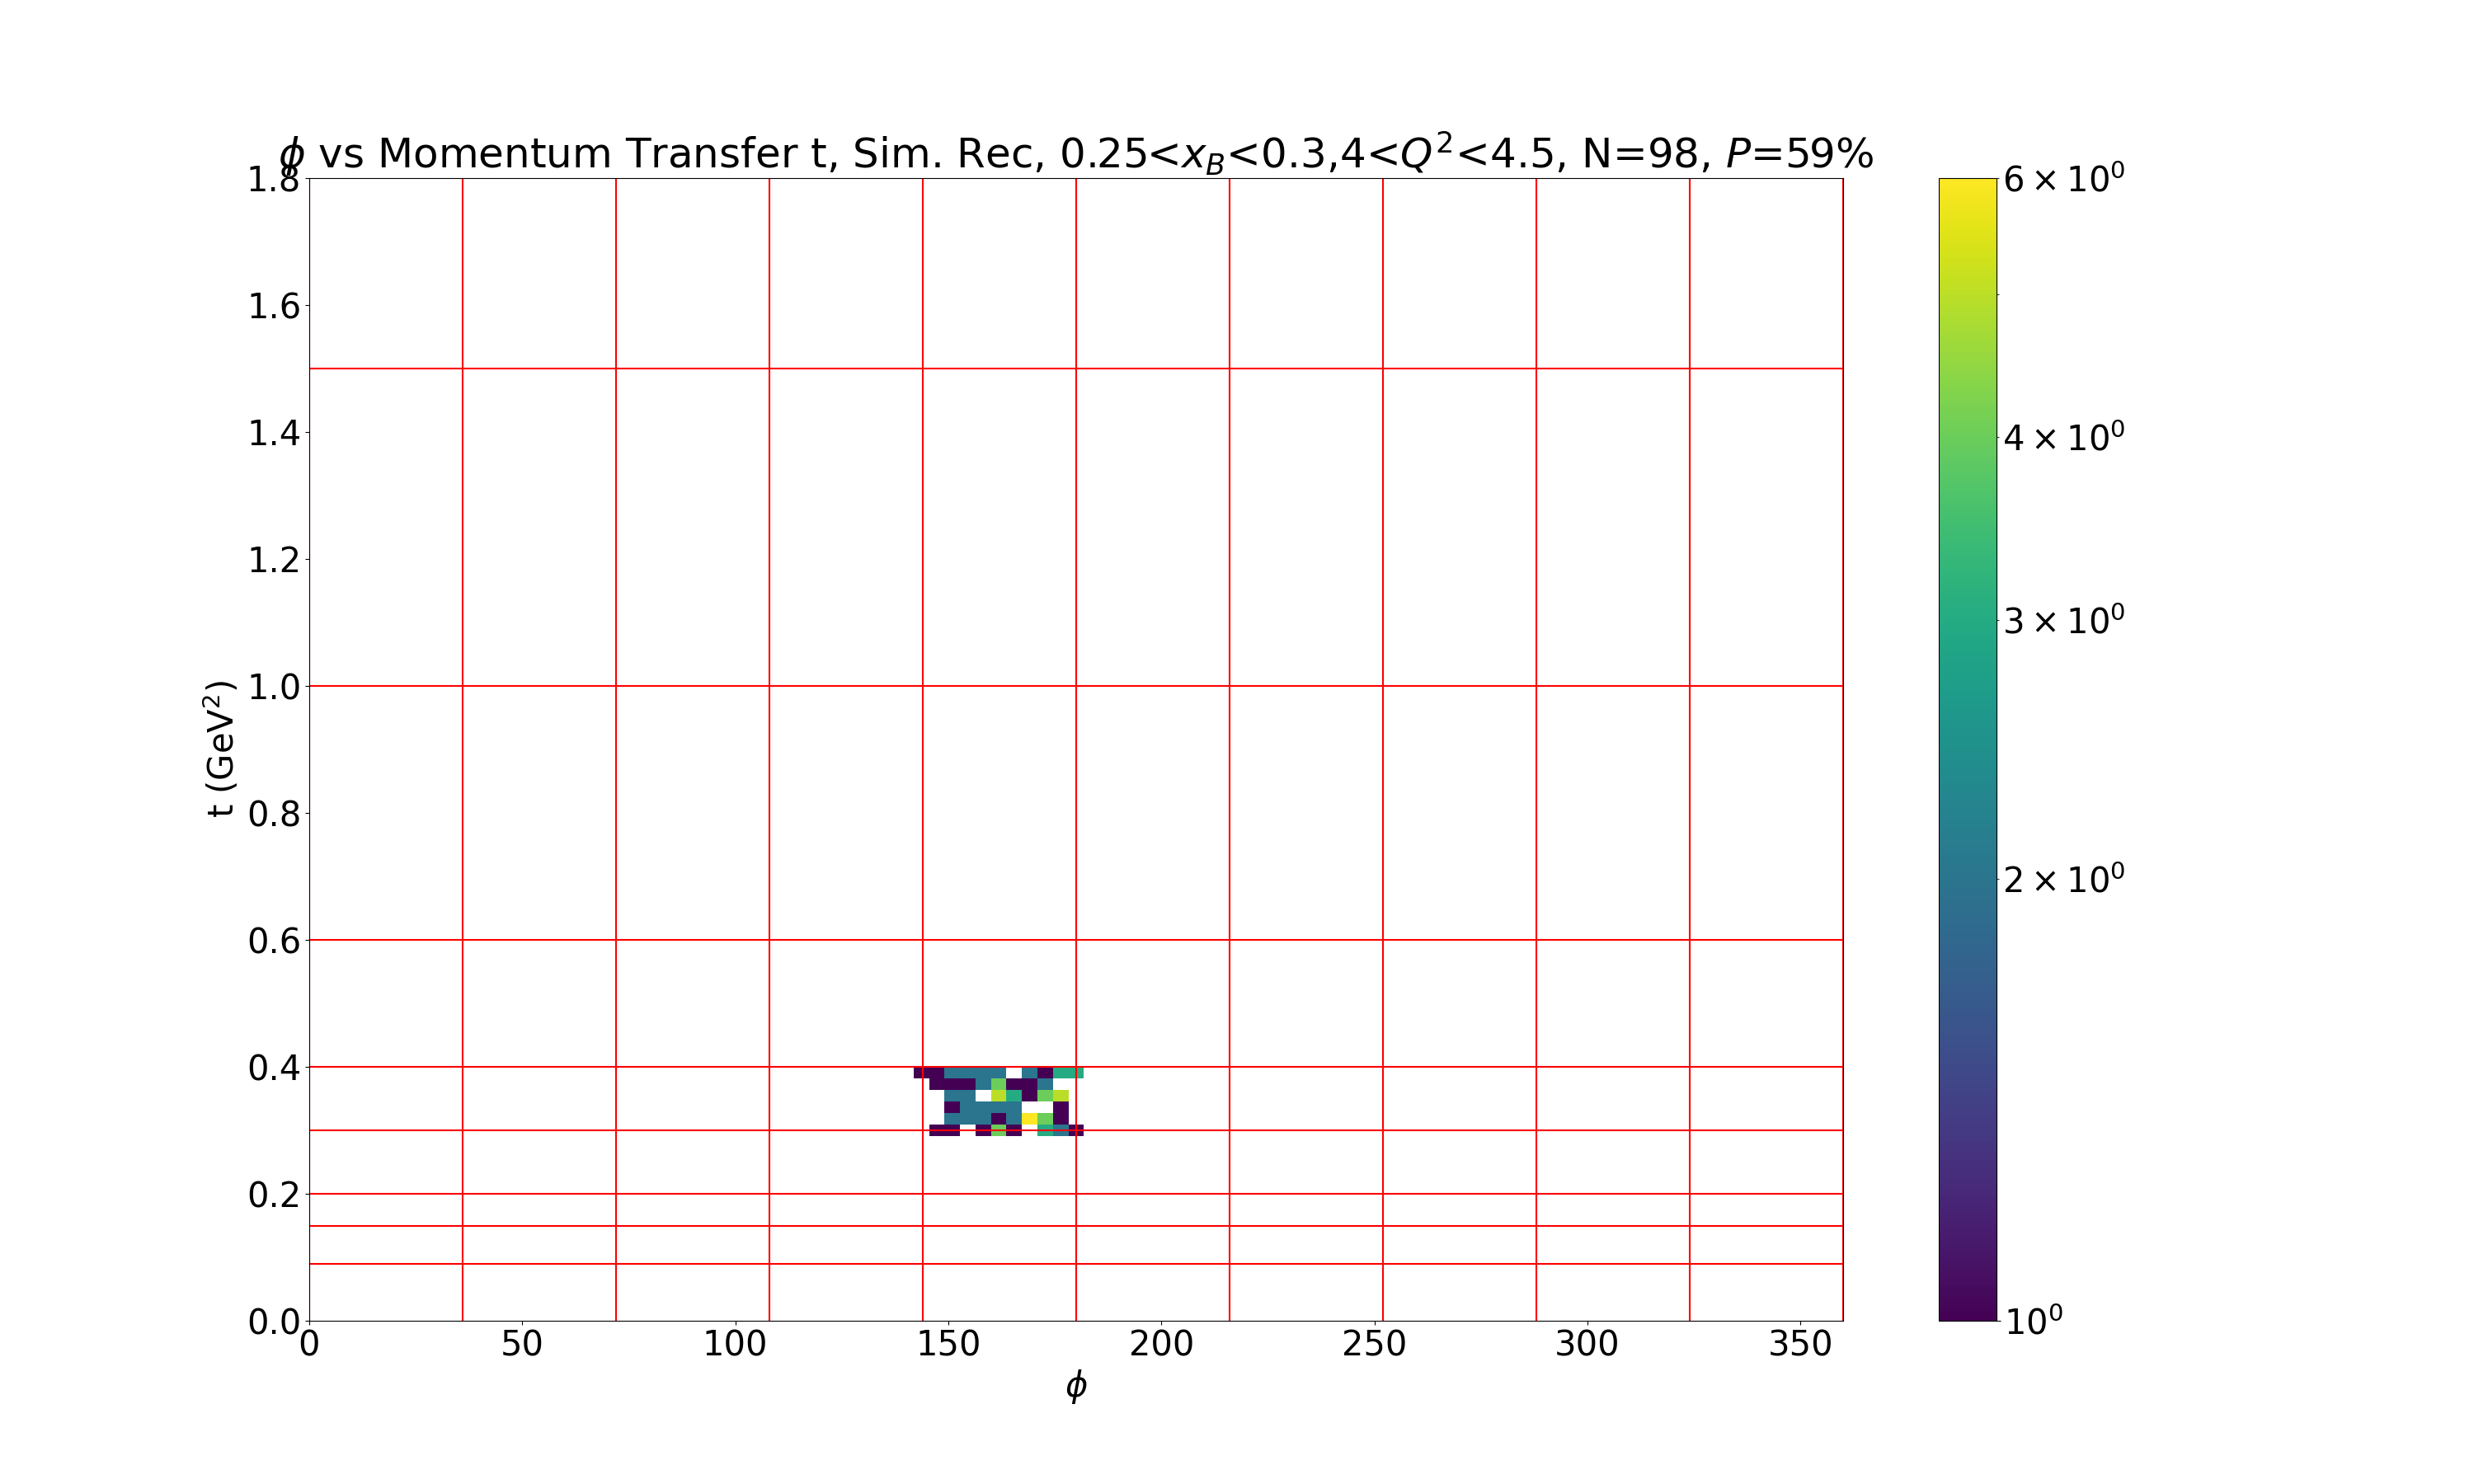
\includegraphics[trim={0 0 17.5cm 6cm},clip,width=0.47\textwidth]{Chapters/Ch5-Further/0_IBU/pics/migration_example/phi_vs_Momentum_Transfer_t,_Sim_Rec,_025x_B03,4Q245,_N=98,_P=59.png}}
        
        \caption[Binning]{Binning. }\label{fig:mig_ex}
    \end{figure}
    
    
    \begin{figure}[ht]
    \centering
    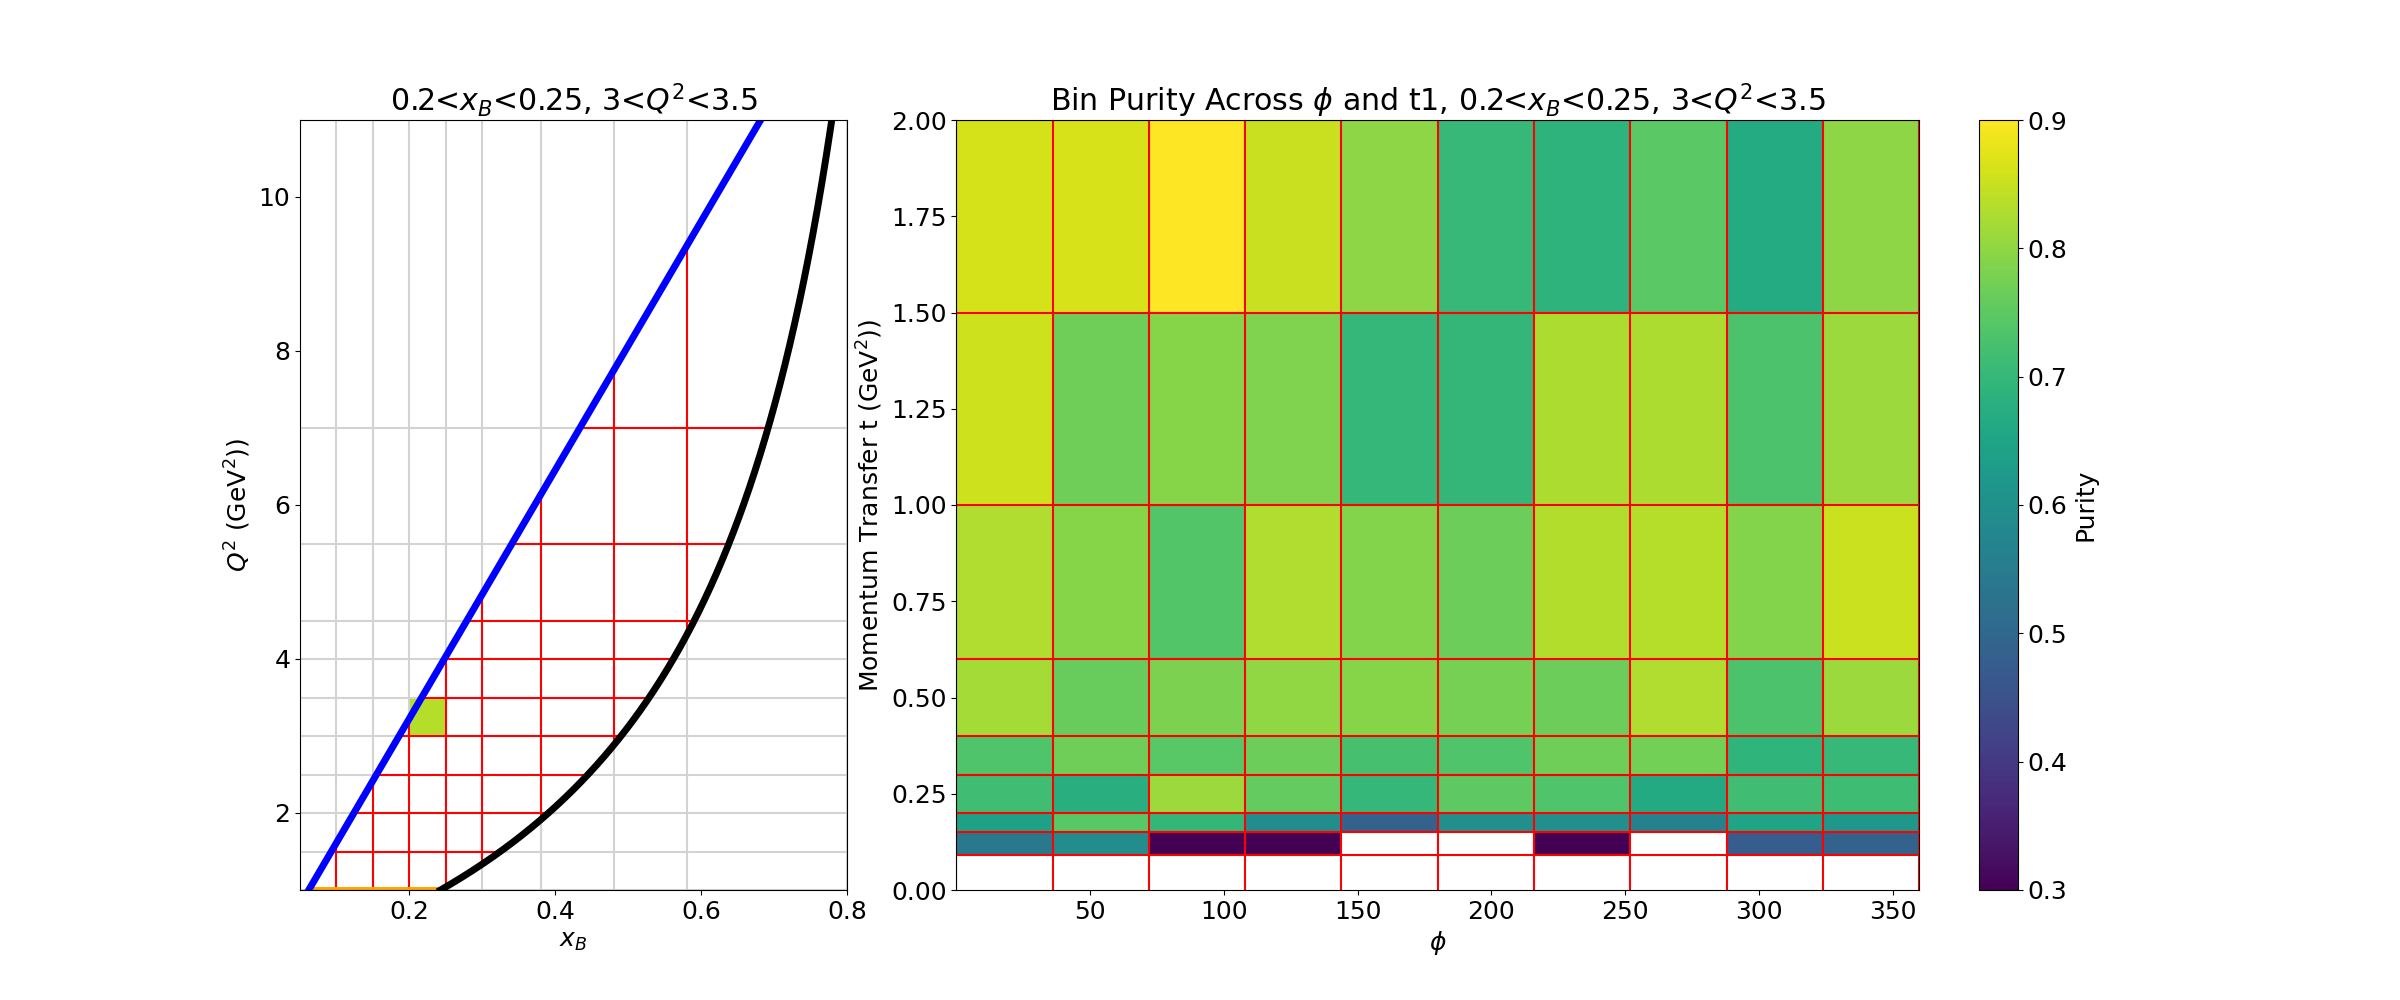
\includegraphics[trim={0 0 0 0},clip,width=\textwidth]{Chapters/Ch5-Further/0_IBU/pics/complete/testfig.png}
    \caption[words]{words}
    \label{fig:ibu5}
    \end{figure}
    
    
    \begin{figure}[H]
        \centering
        \subfloat[xb vs q2]{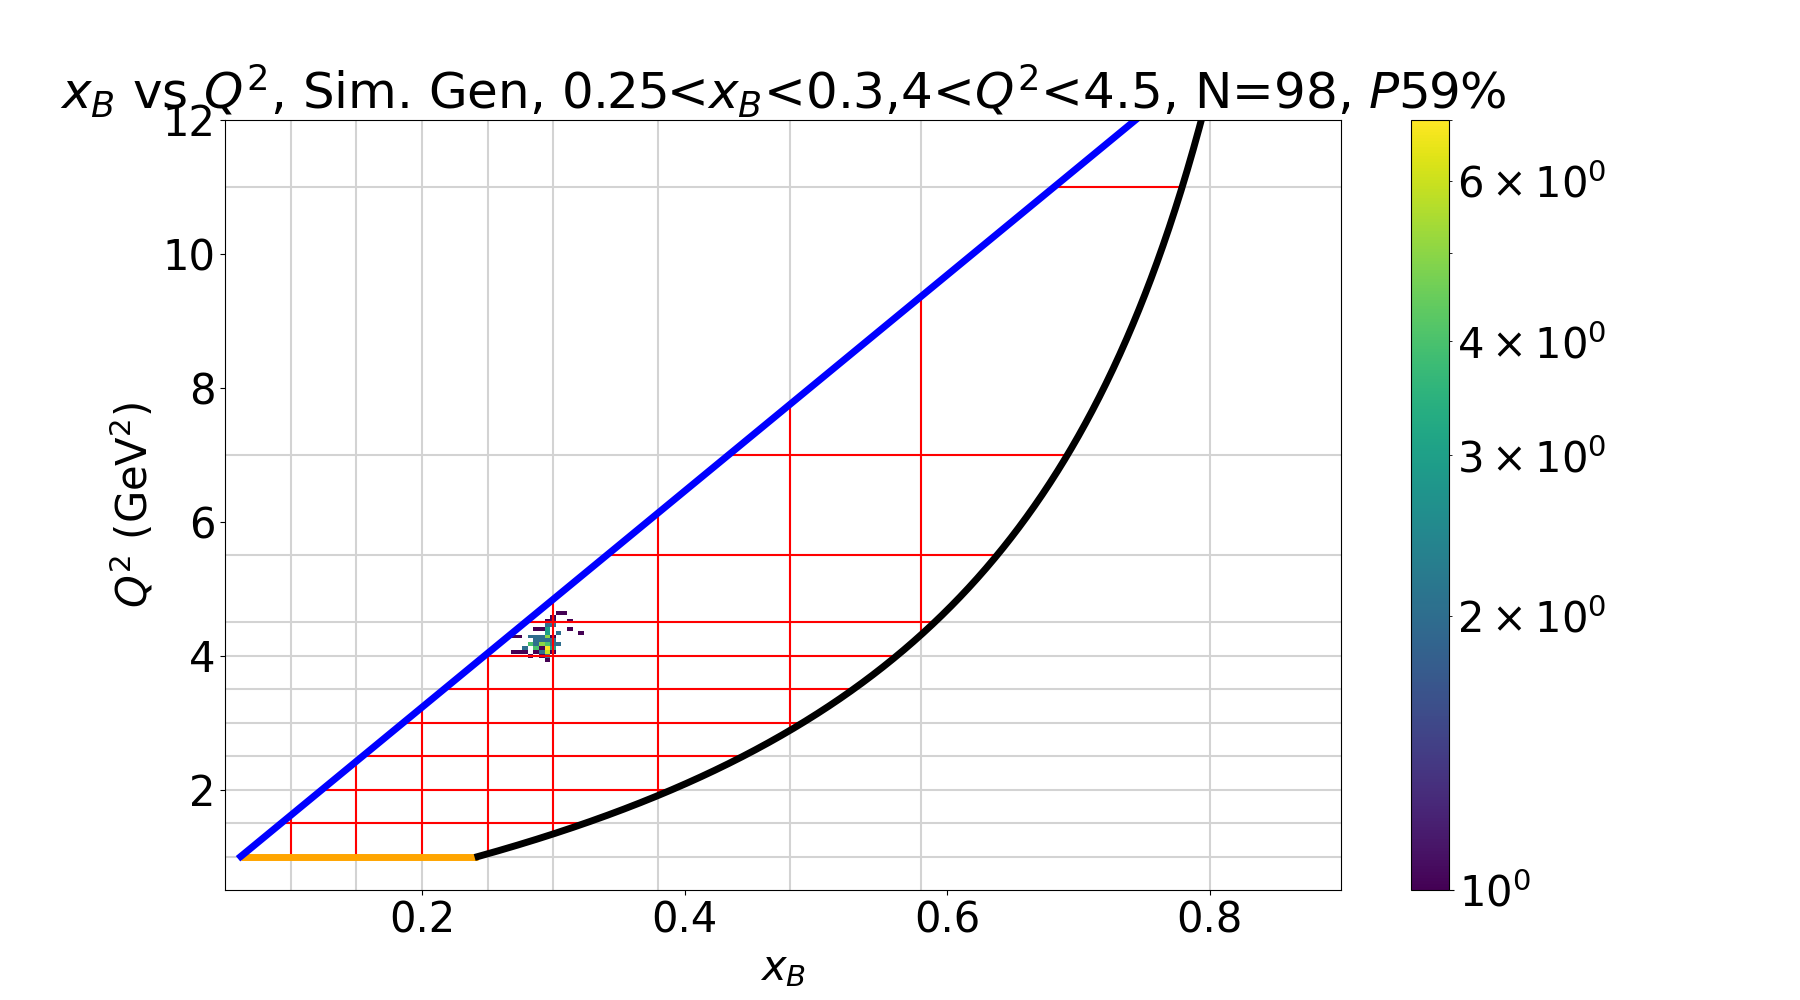
\includegraphics[trim={0 0 10cm 3.5cm},clip,width=0.52\textwidth]{Chapters/Ch5-Further/0_IBU/pics/migration_example/x_B_vs_Q2,_Sim_Gen,_025x_B03,4Q245,_N=98,_P59.png}}
        \hfill
        \subfloat[phi vs t]{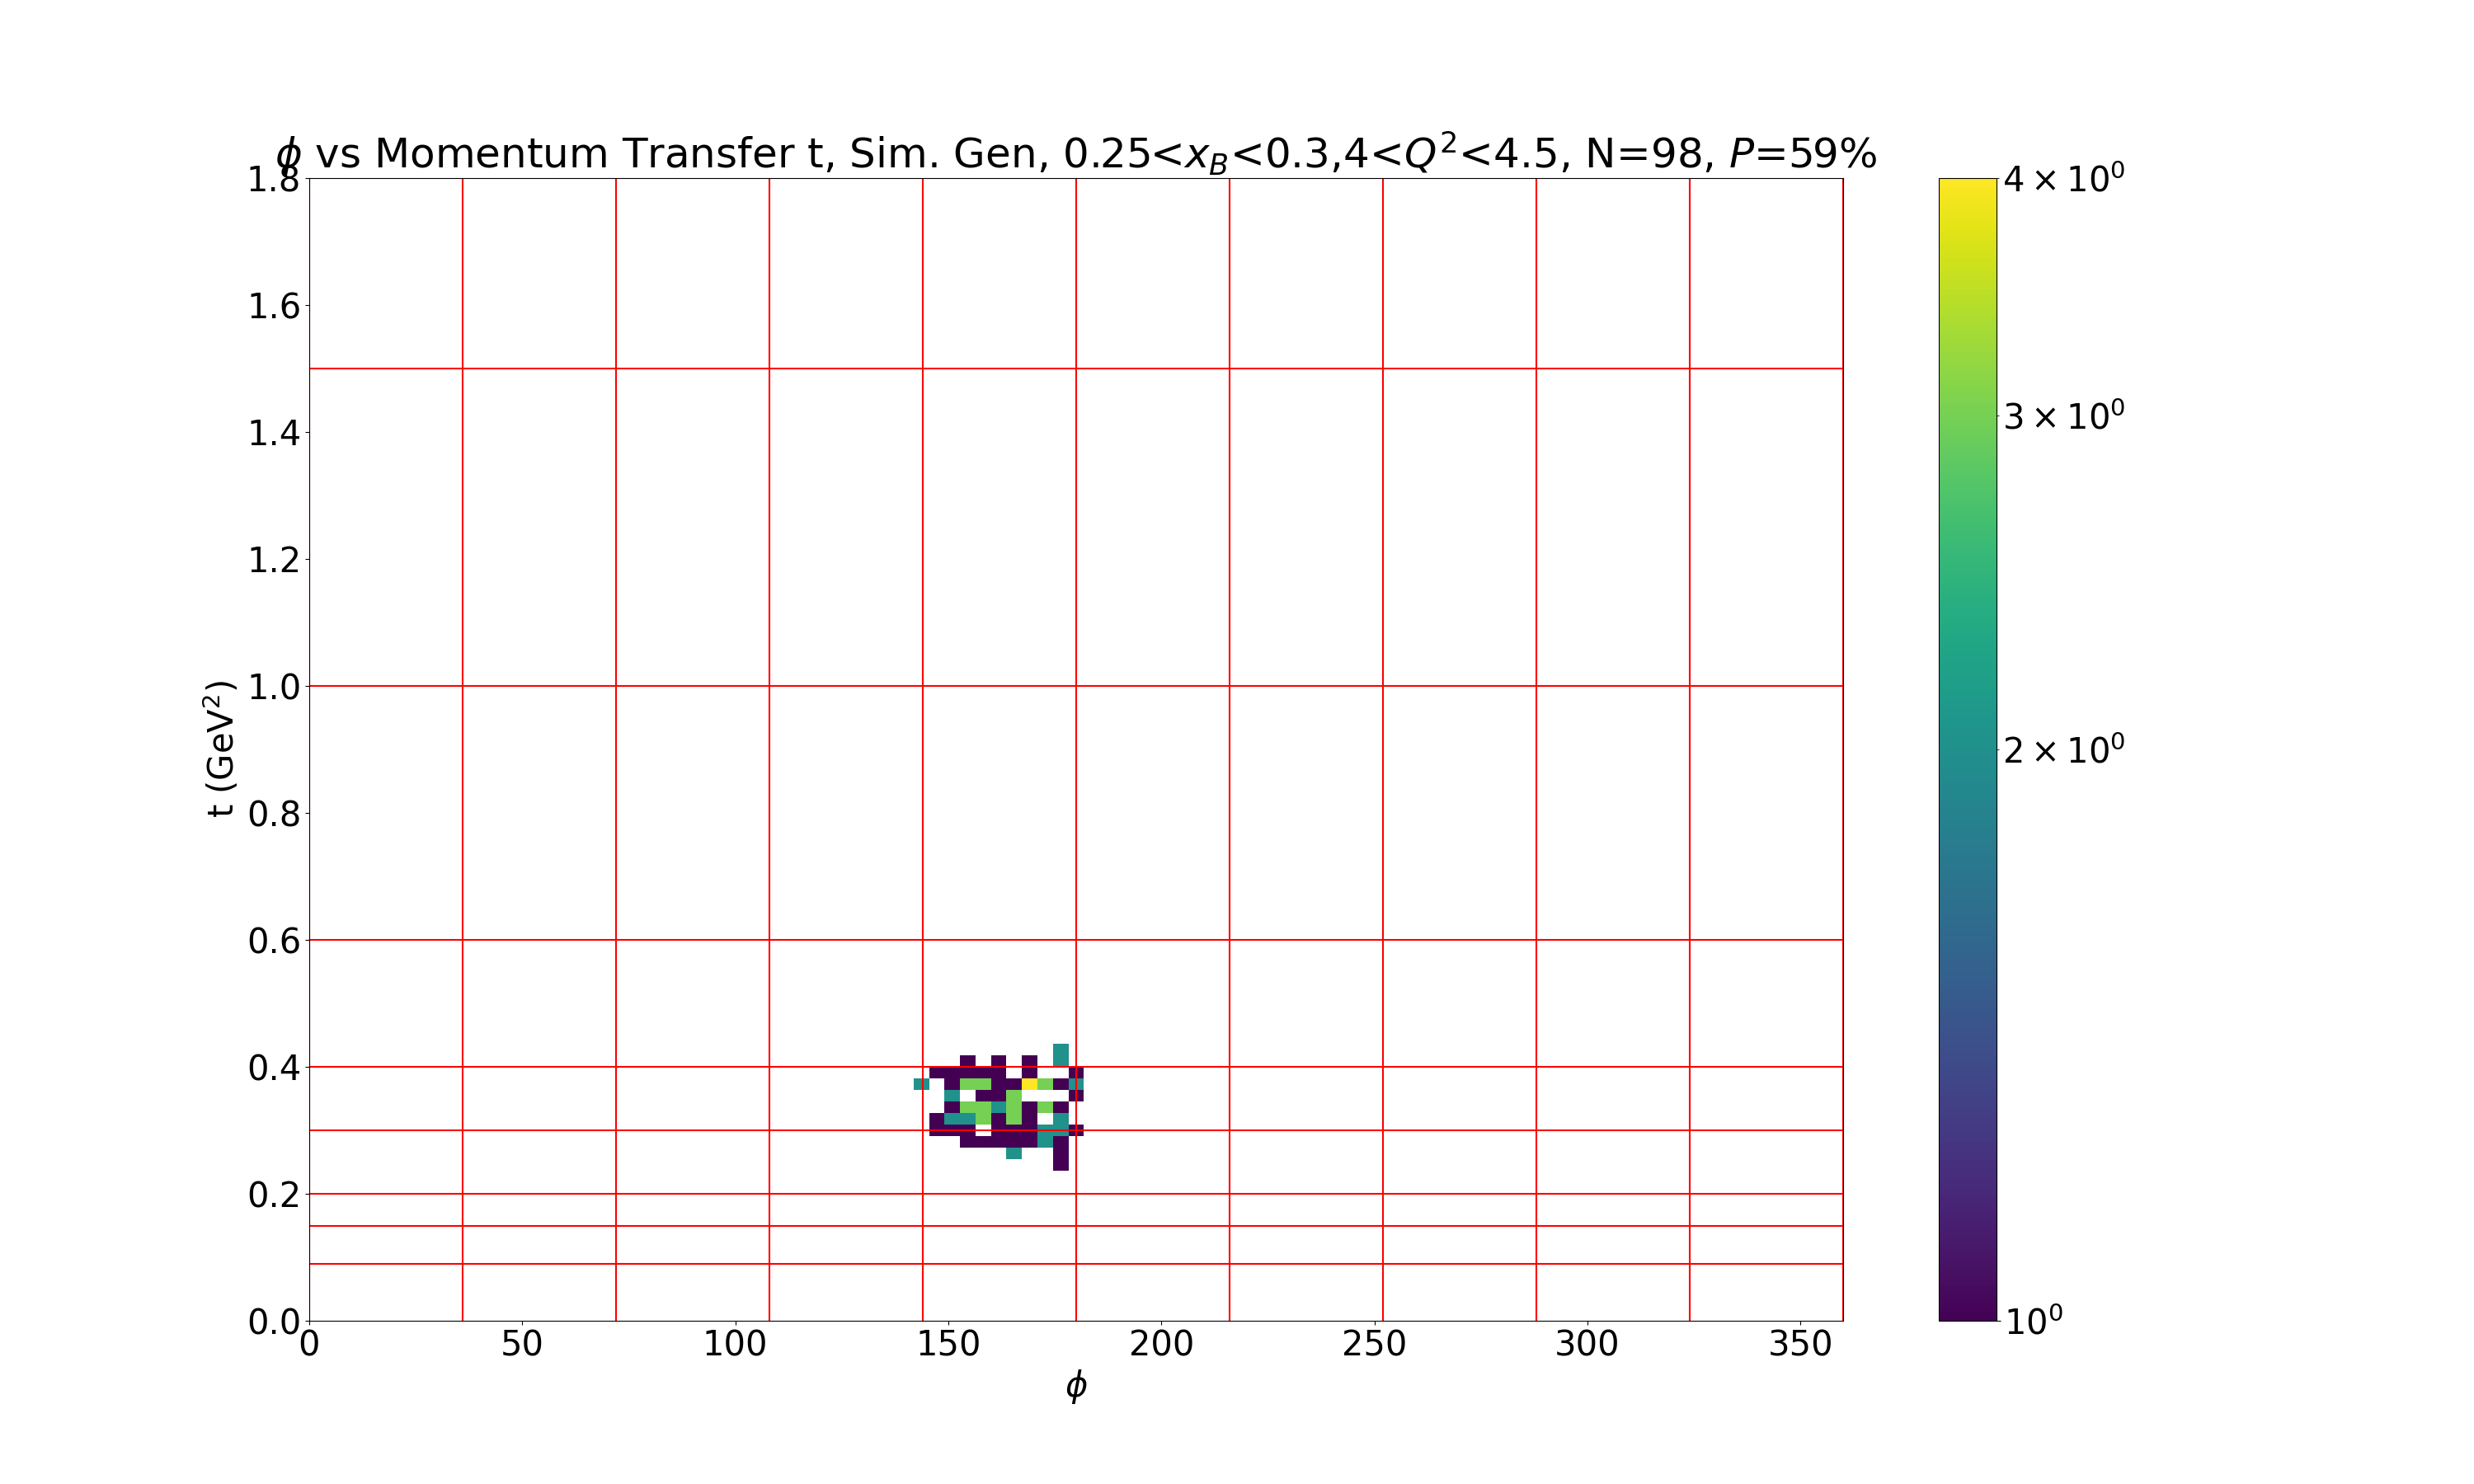
\includegraphics[trim={0 0 17.5cm 6cm},clip,width=0.47\textwidth]{Chapters/Ch5-Further/0_IBU/pics/migration_example/phi_vs_Momentum_Transfer_t,_Sim_Gen,_025x_B03,4Q245,_N=98,_P=59.png}}
        
        \caption[Reduced Cross Sections Across $\phi$]{Reduced cross sections across $\phi$ at (a) low kinematics and (b) high kinematics. Where kinematic overlap exists, the CLAS6 result \parencite{Bedlinskiy2014ExclusiveCLAS} is shown in blue with an error band (in modified form to account for beam energy differences). }\label{fig:mig_ex}
        %\caption[Reduced Cross Sections Across $\phi$]{Reduced Cross Sections Across $\phi$}
    \end{figure}
    
    
    From this, we can calculate the bin purity and efficency of each bin, giving us for example
    
    
    \begin{figure}[ht]
    \centering
    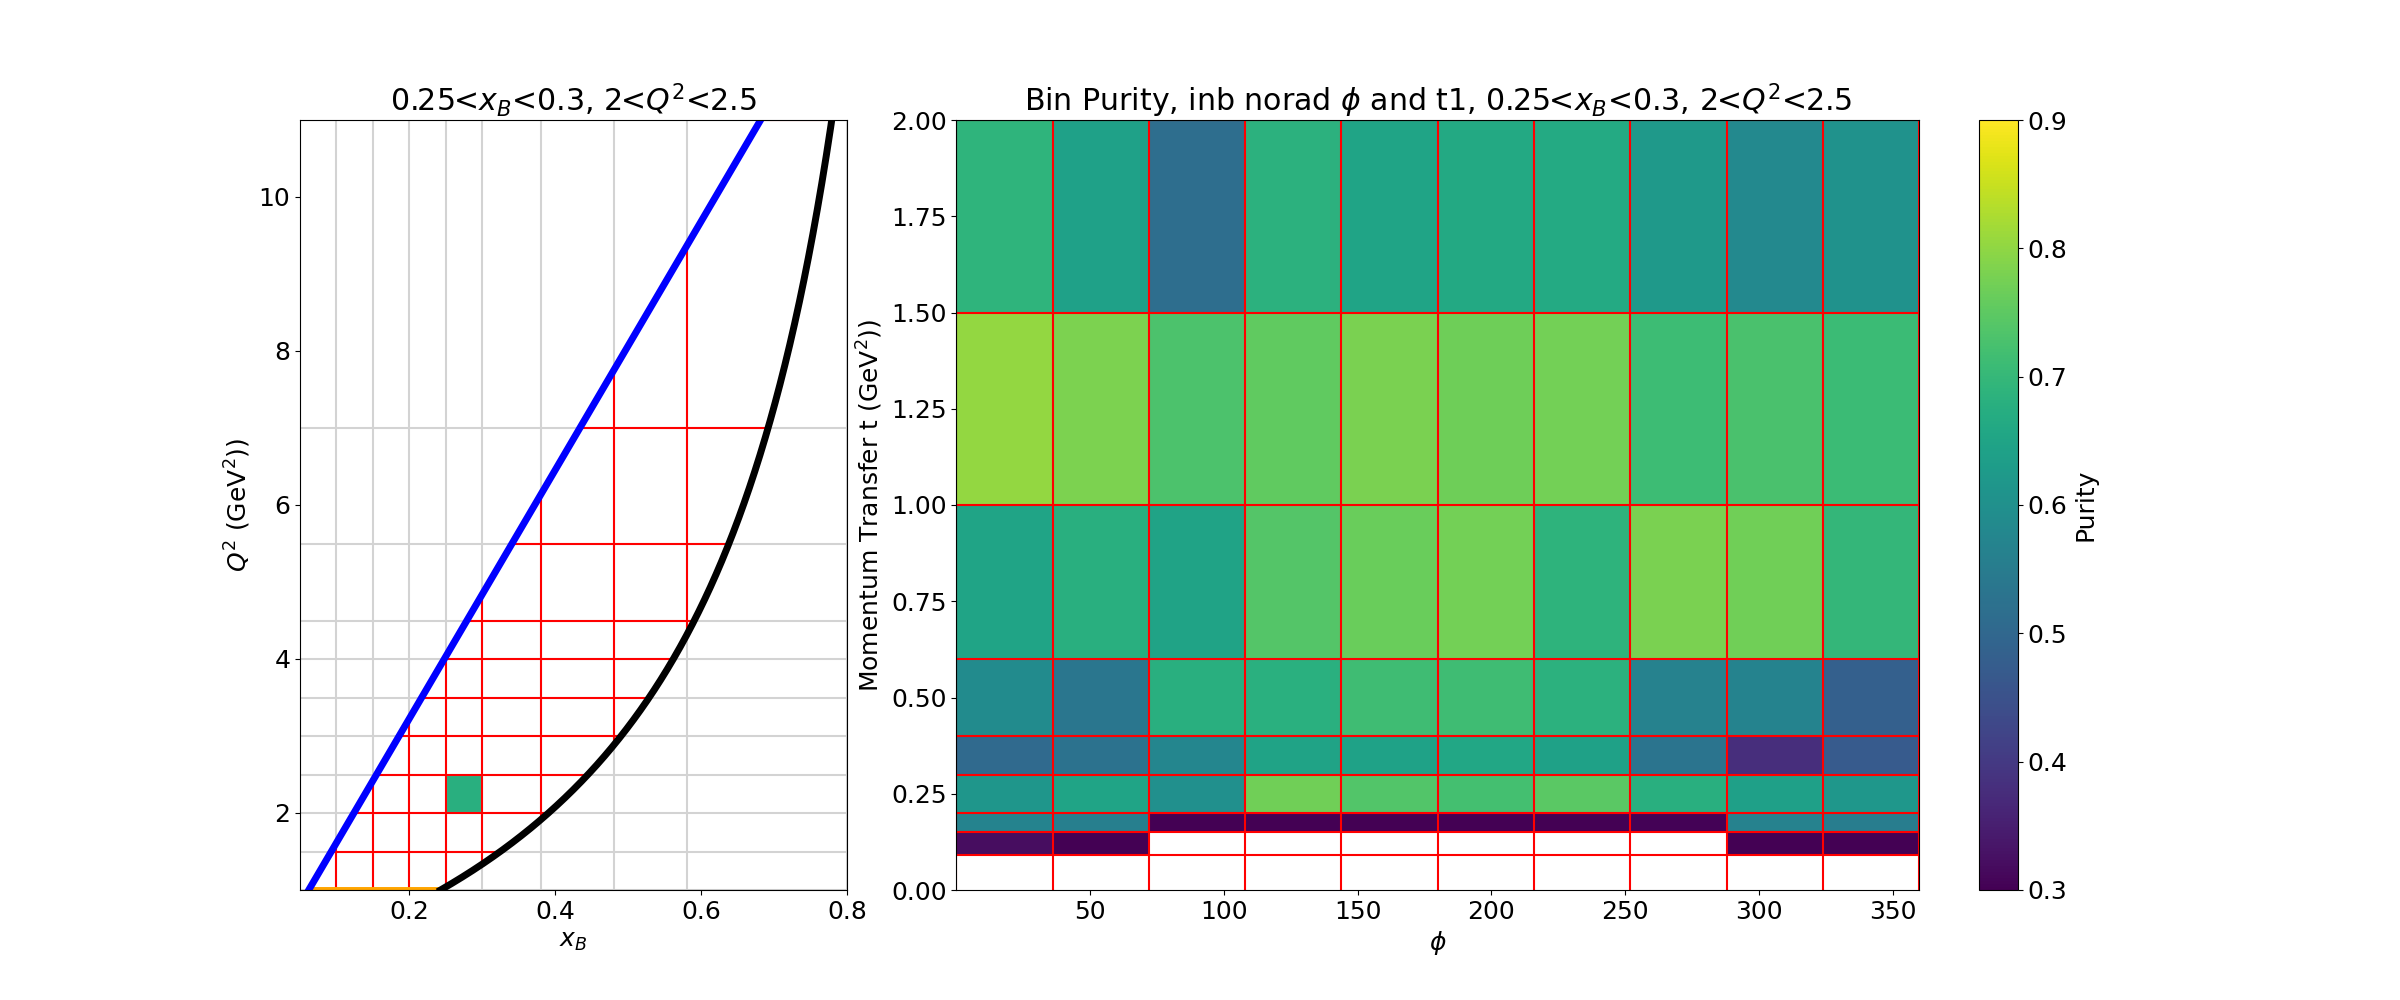
\includegraphics[trim={0 0 0 0},clip,width=\textwidth]{Chapters/Ch5-Further/0_IBU/pics/purities/inb_norad_t1/bin_purity_0.25_0.3_2_2.5.png}
    \caption[words]{words}
    \label{fig:ibu10}
    \end{figure}
    
    
    We can plot all of them as:
    
    
    \begin{figure}[ht]
    \centering
    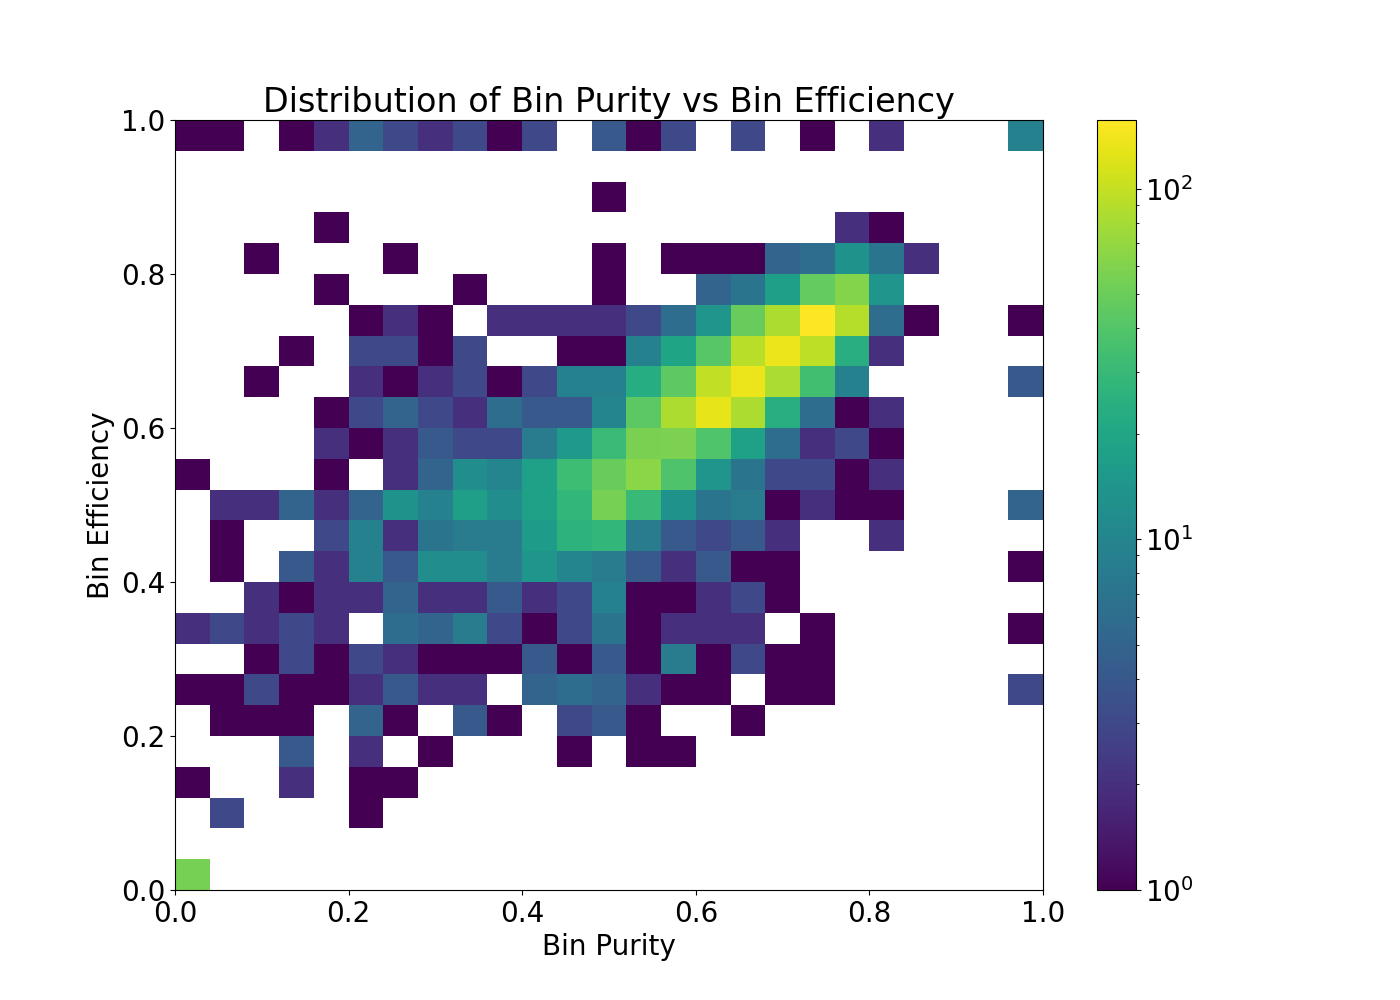
\includegraphics[trim={0 0 0 0},clip,width=\textwidth]{Chapters/Ch5-Further/0_IBU/pics/overview/t1_bin_purity_vs_bin_efficiency.png}
    \caption[words]{words}
    \label{fig:ibu10}
    \end{figure}

    By superimposing a periodic waving to illustrate point locality, we can observe drifts between generated and reconstructed positions. There is no systematic shift, and improvements to base reconstruction code are currently being developed as part of a collaboration-wide effort. 
    
    \begin{figure}[ht]
        \centering
        \subfloat[][Caption 1]{
        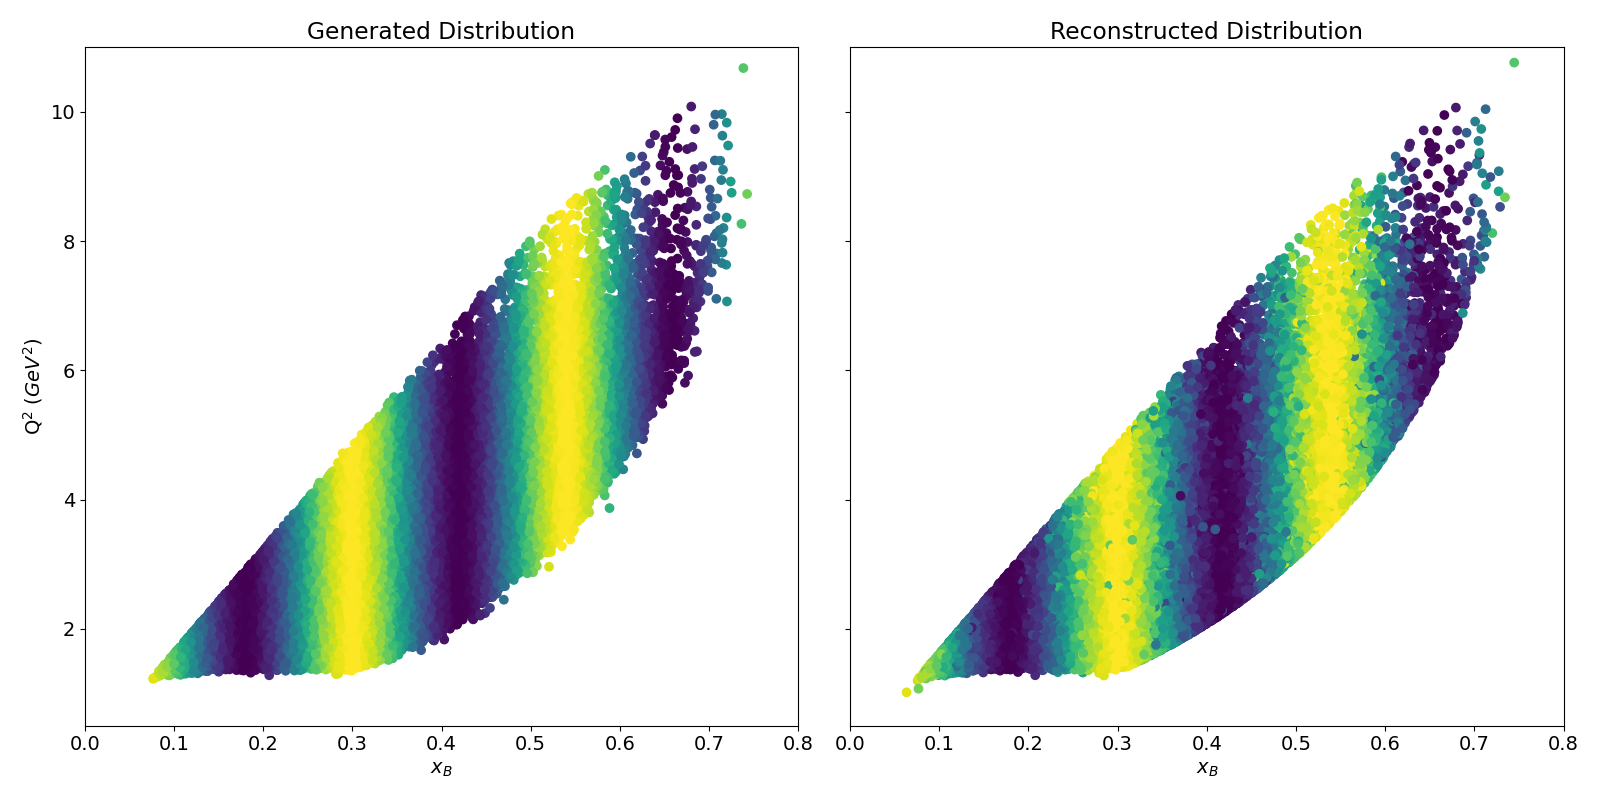
\includegraphics[width=0.45\textwidth]{Chapters/Ch5-Further/0_IBU/pics/waving/sine_plots_xB.png}
        \label{fig:ibu4a}}
        \hfill
        \subfloat[][Caption 2]{
        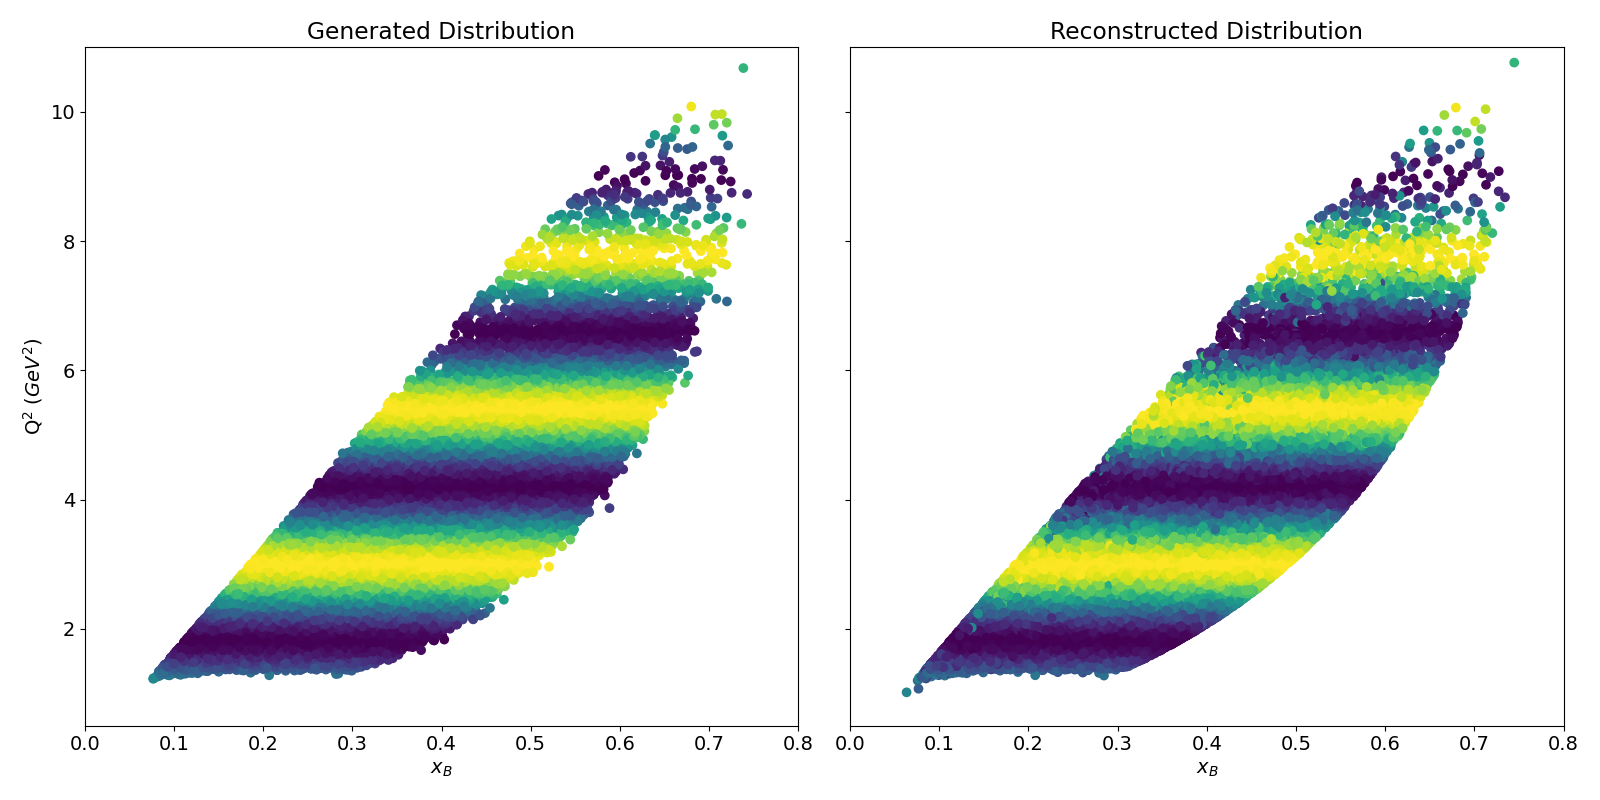
\includegraphics[width=0.45\textwidth]{Chapters/Ch5-Further/0_IBU/pics/waving/sine_plots_Q2.png}
        \label{fig:ibu4b}}
        \\
        \subfloat[][Caption 3]{
        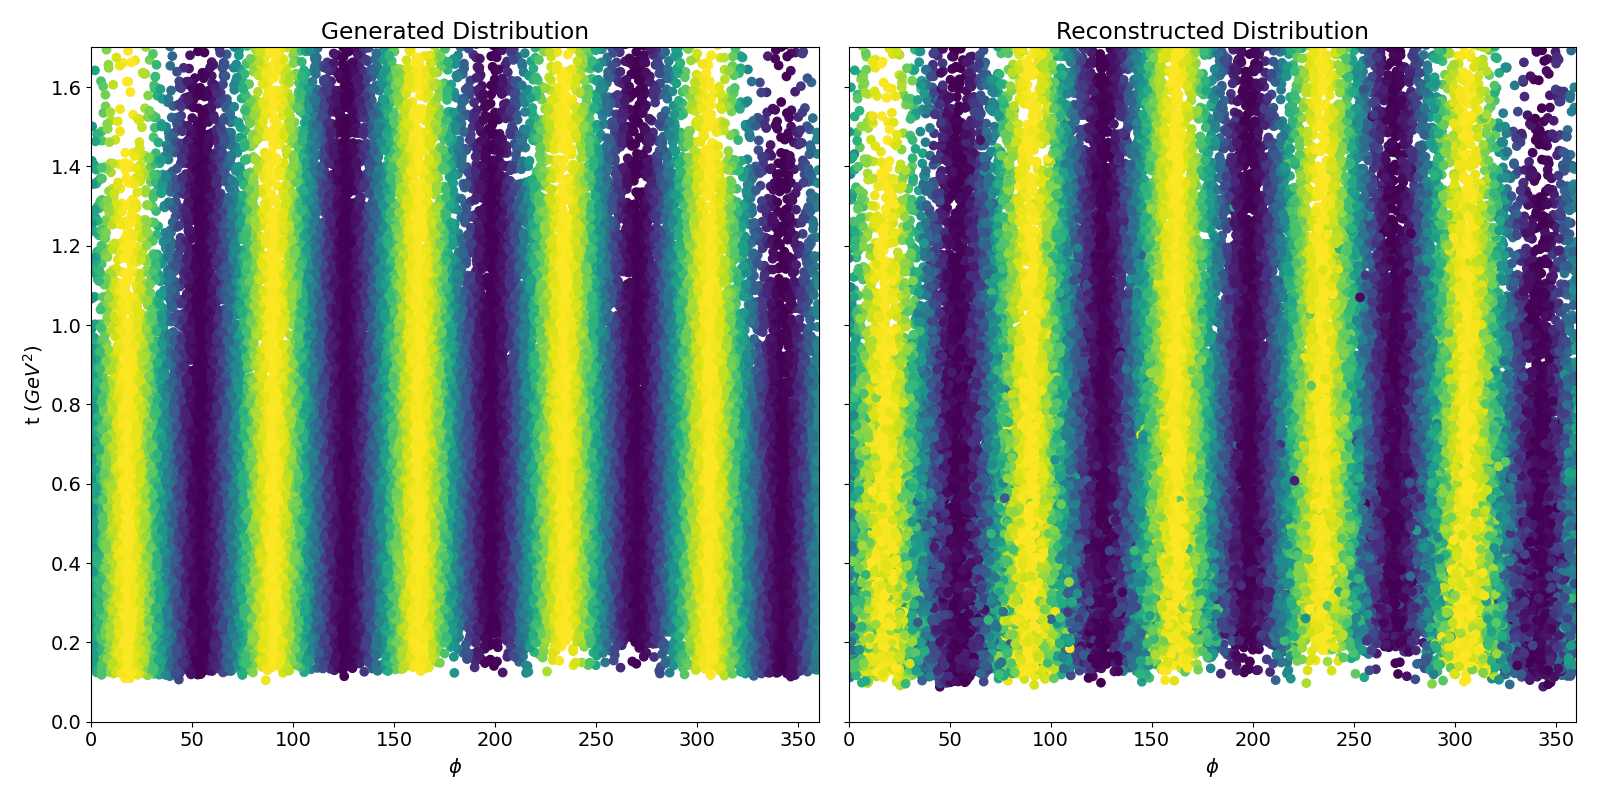
\includegraphics[width=0.45\textwidth]{Chapters/Ch5-Further/0_IBU/pics/waving/sine_plots_phi.png}
        \label{fig:ibu4c}}
        \hfill
        \subfloat[][Caption 4]{
        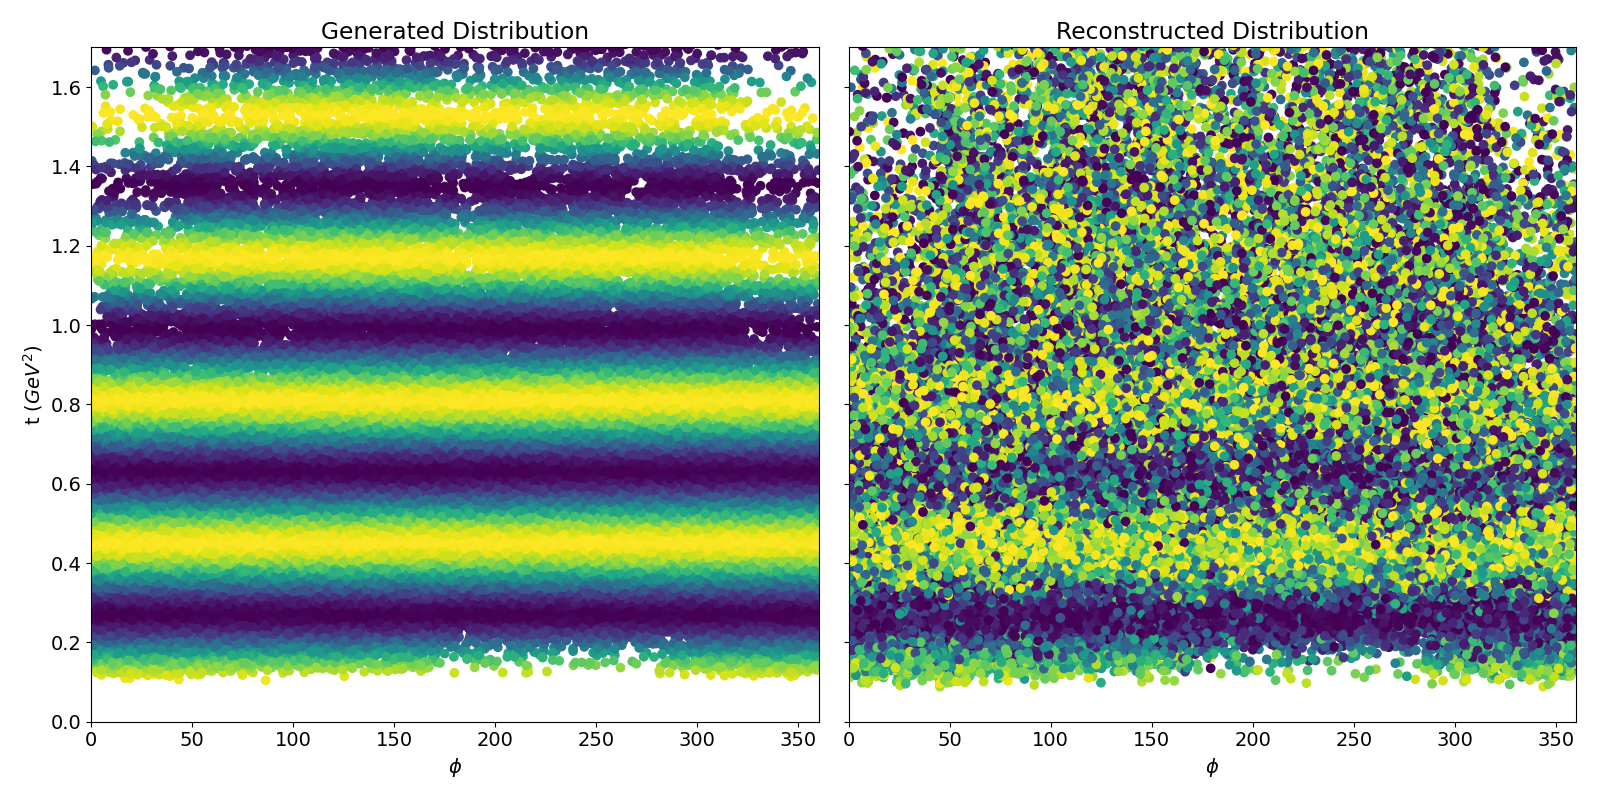
\includegraphics[width=0.45\textwidth]{Chapters/Ch5-Further/0_IBU/pics/waving/sine_plots_t.png}
        \label{fig:ibu4d}}
        \caption{Overall Caption for all figures}
        \label{fig:ibu4}
    \end{figure}
    

    Could index off of t2 missing mass, but not ideal for radiative corrections and in general want 
    
    \begin{figure}[ht]
        \centering
        \subfloat[][Caption 1]{
        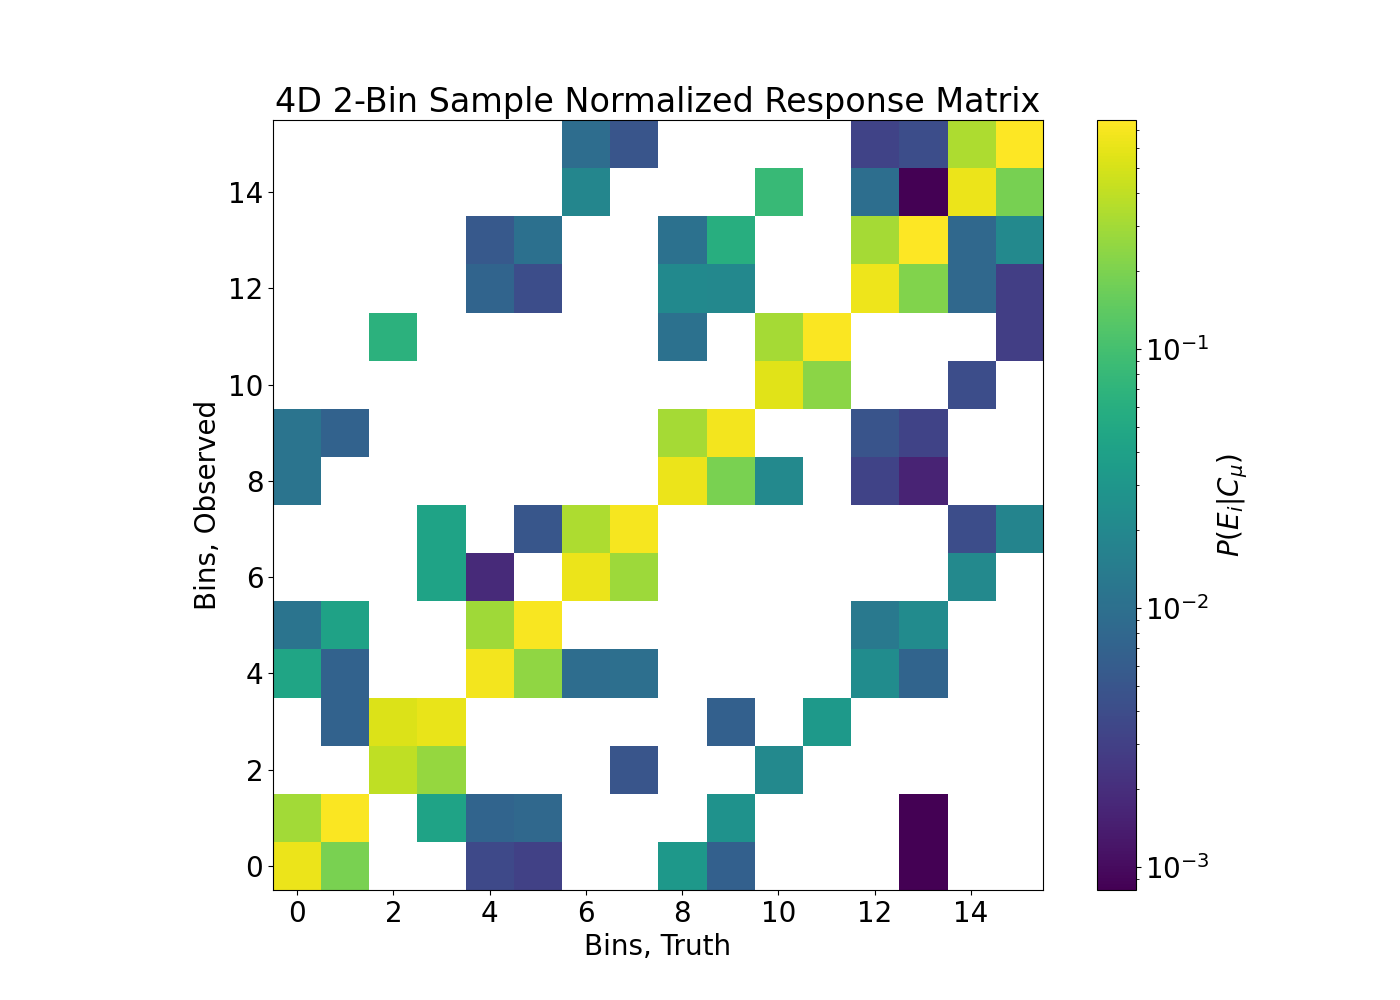
\includegraphics[width=0.45\textwidth]{Chapters/Ch5-Further/0_IBU/pics/4d-2n_example/4D_2bin_sample_normalized_response_matrix.png}
        \label{fig:ibu4a}}
        \hfill
        \subfloat[][Caption 2]{
        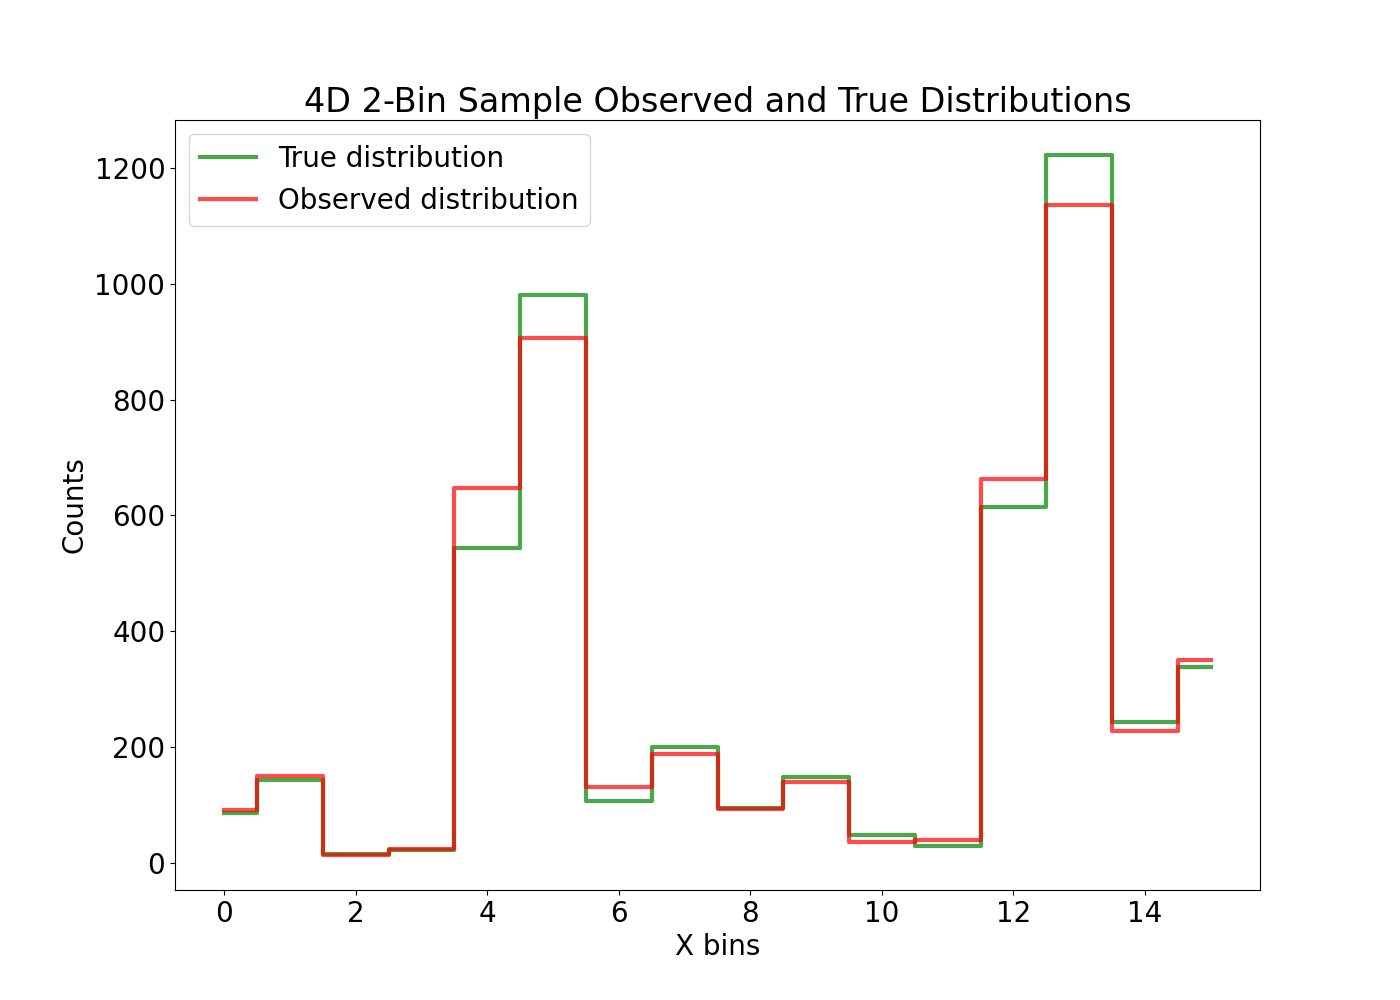
\includegraphics[width=0.45\textwidth]{Chapters/Ch5-Further/0_IBU/pics/4d-2n_example/4D_2bin_sample_observed_and_true_distributions.png}
        \label{fig:ibu4b}}
        \\
        \subfloat[][Caption 3]{
        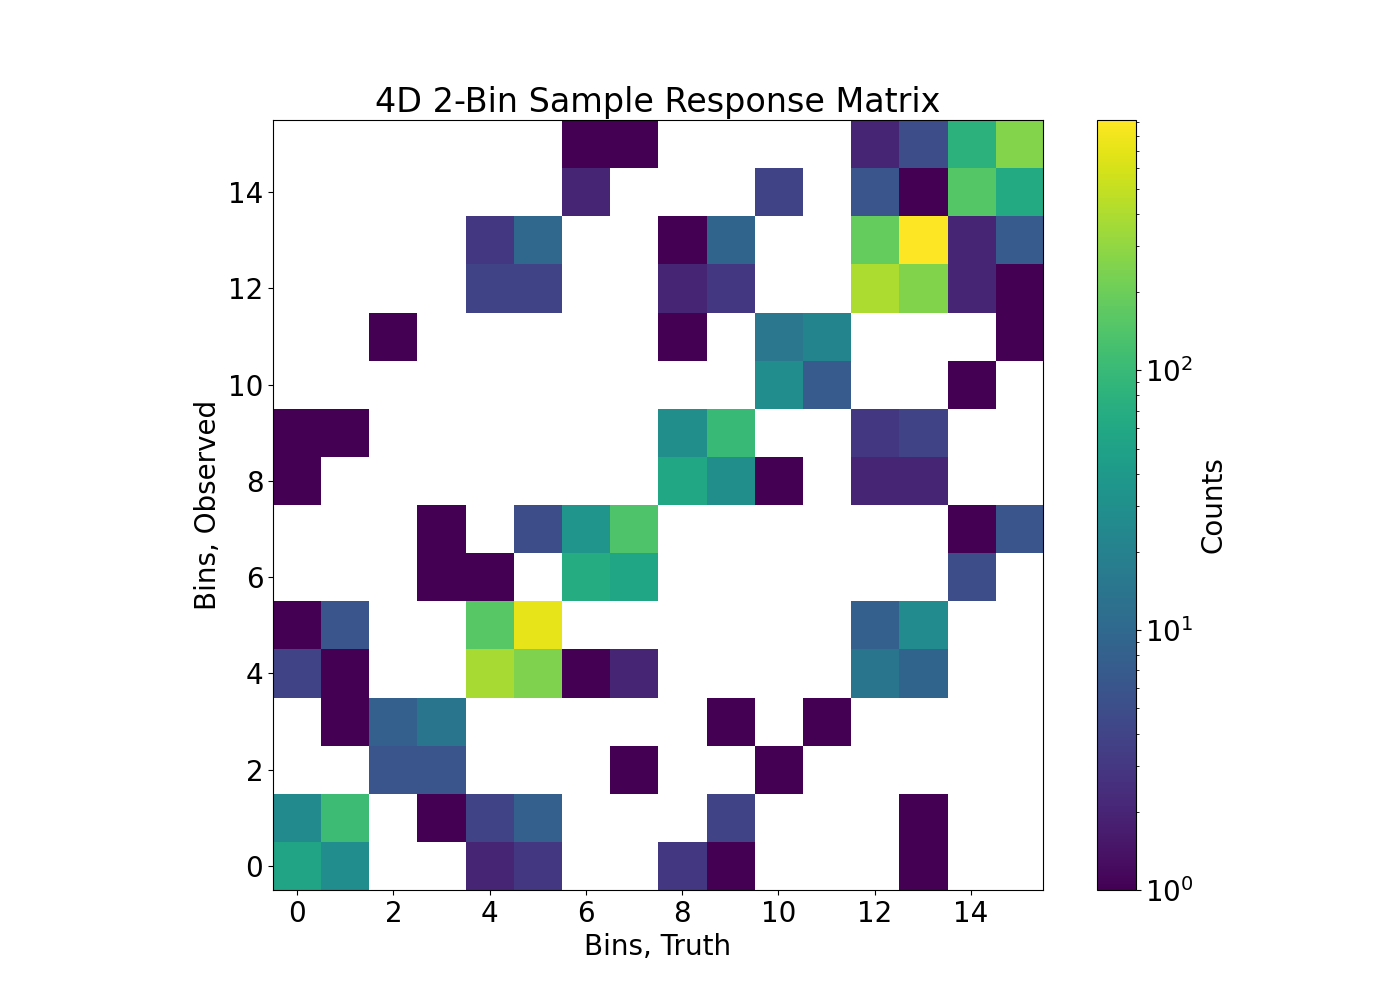
\includegraphics[width=0.45\textwidth]{Chapters/Ch5-Further/0_IBU/pics/4d-2n_example/4D_2bin_sample_response_matrix.png}
        \label{fig:ibu4c}}
        \hfill
        \subfloat[][Caption 4]{
        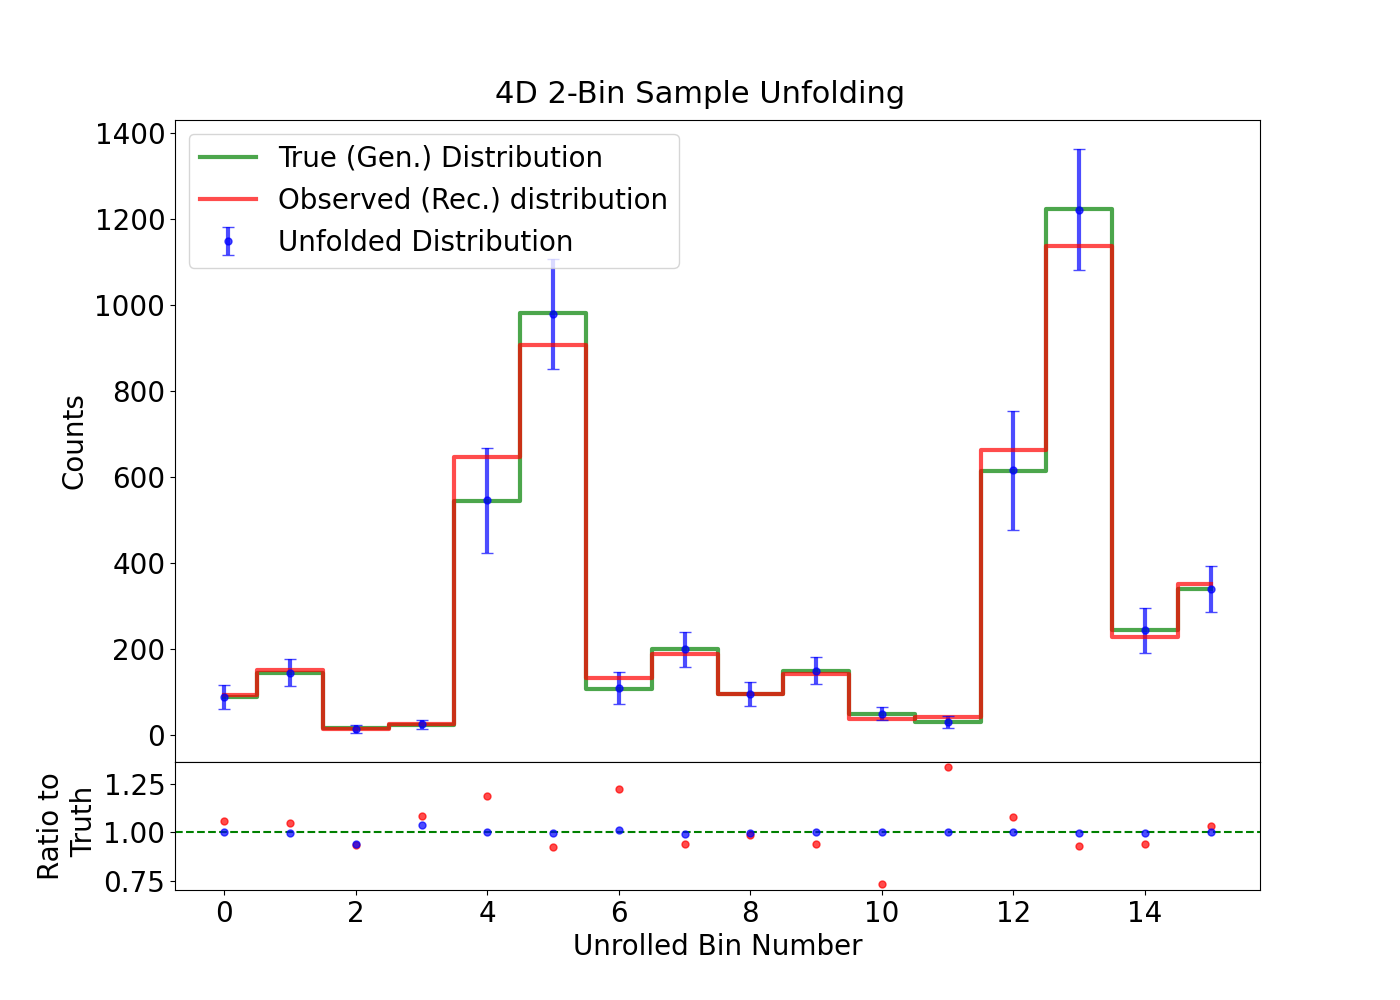
\includegraphics[width=0.45\textwidth]{Chapters/Ch5-Further/0_IBU/pics/4d-2n_example/4D_2bin_sample_unfolding.png}
        \label{fig:ibu4d}}
        \caption{Overall Caption for all figures}
        \label{fig:ibu4}
    \end{figure}
    
    
    
    
    \begin{figure}
        \centering
        \subfloat[][4D 2-Bin Sample Response Matrix xb]{
        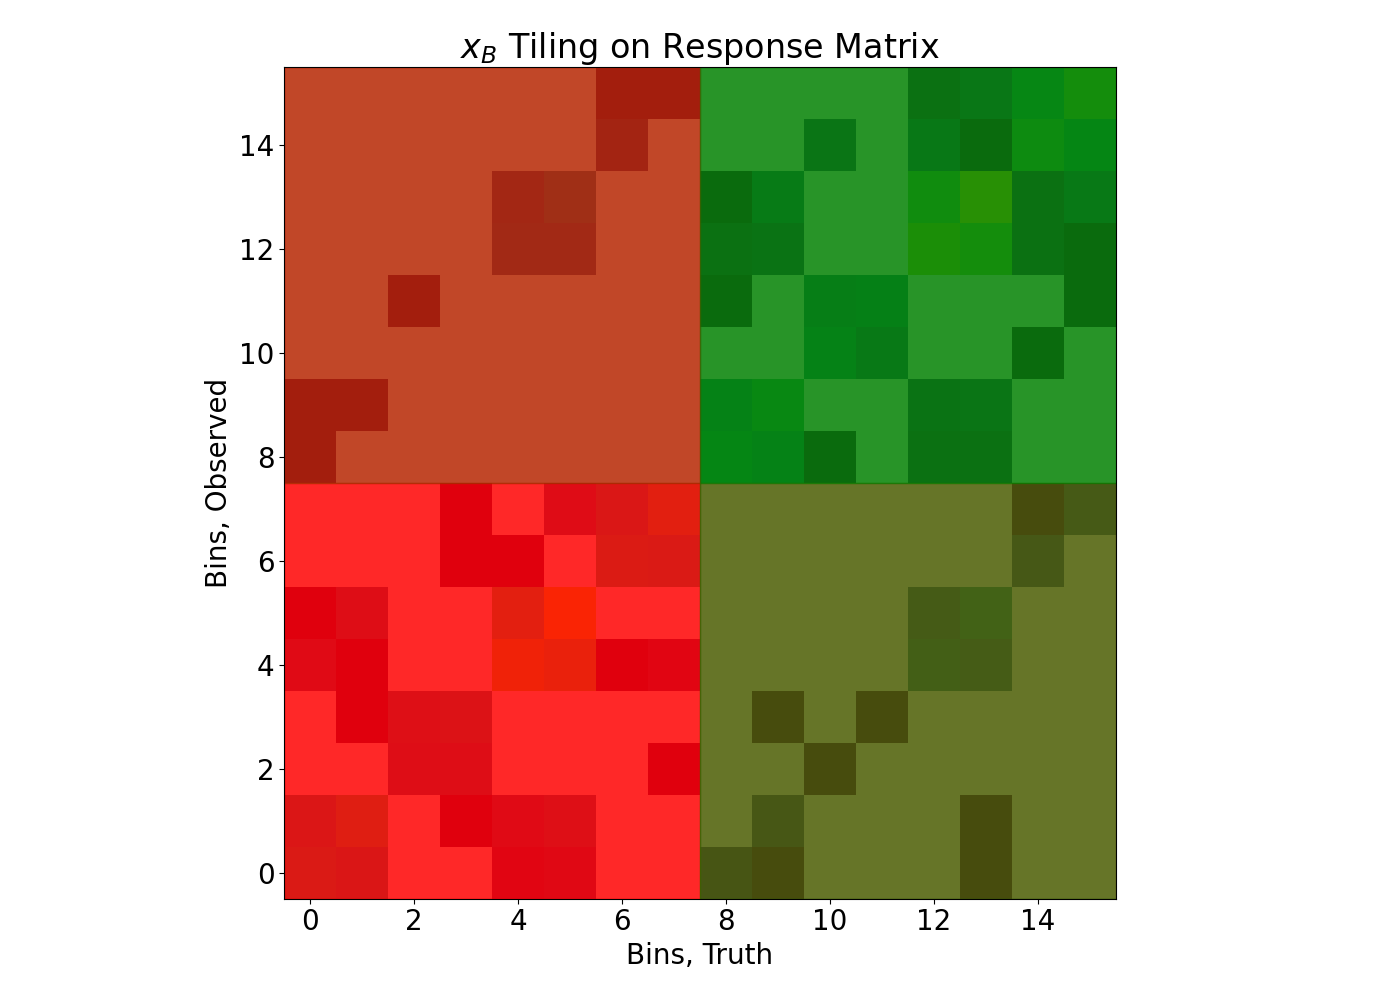
\includegraphics[width=0.45\textwidth]{Chapters/Ch5-Further/0_IBU/pics/4d-2n_example/plaid/4D_2bin_sample_response_matrix_xb.png}
        \label{fig:response_matrix_xb}}
        \hfill
        \subfloat[][4D 2-Bin Sample Response Matrix xb q2]{
        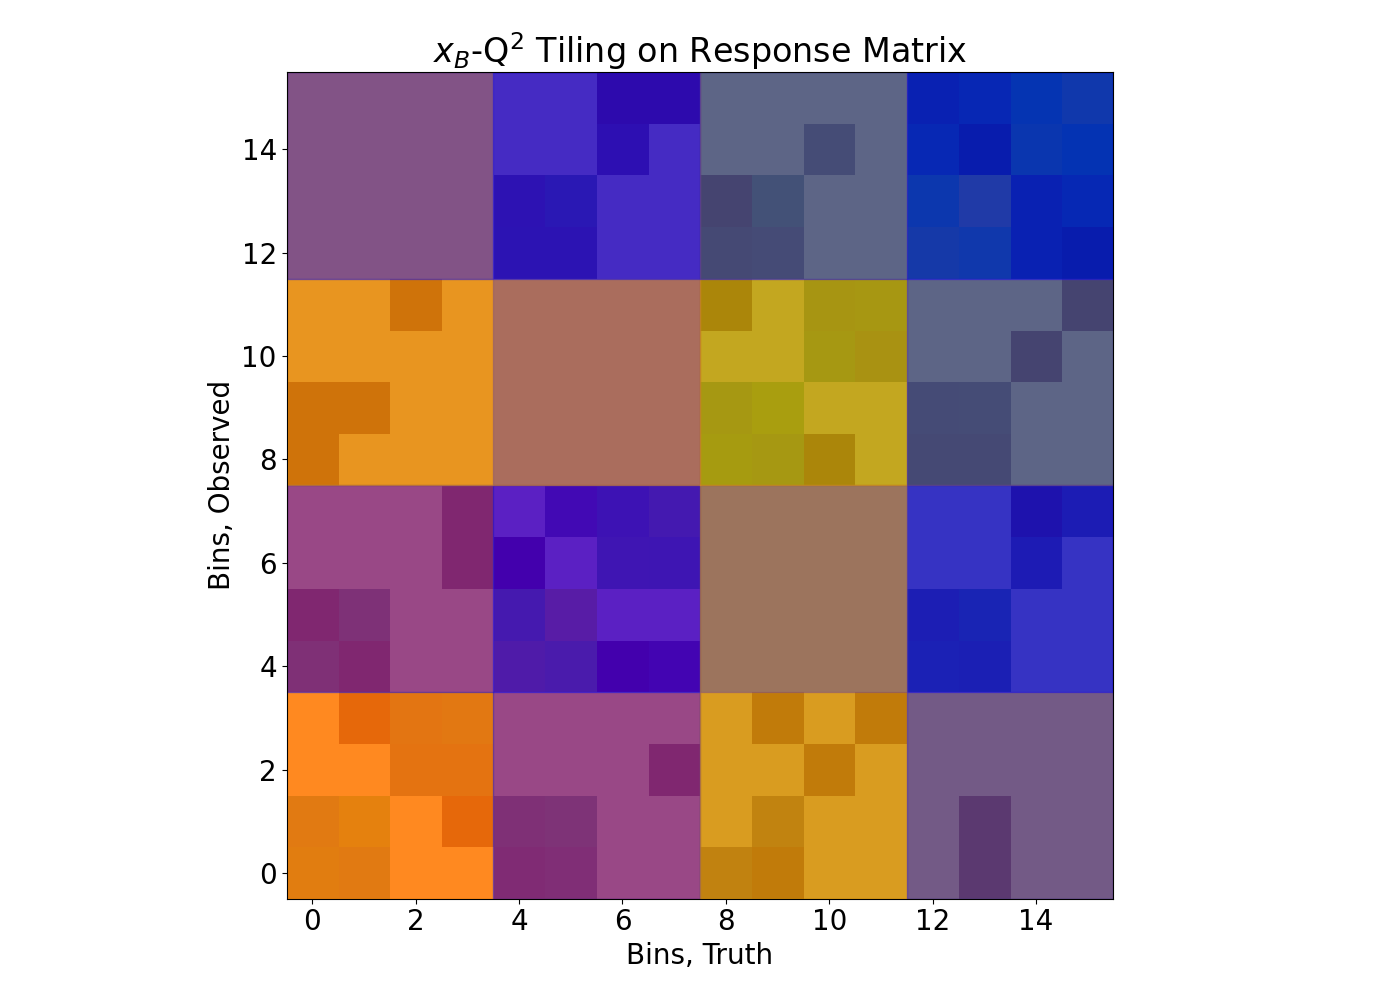
\includegraphics[width=0.45\textwidth]{Chapters/Ch5-Further/0_IBU/pics/4d-2n_example/plaid/4D_2bin_sample_response_matrix_xb_q2.png}
        \label{fig:response_matrix_xb_q2}}
        \\
        \subfloat[][4D 2-Bin Sample Response Matrix xb q2 phi]{
        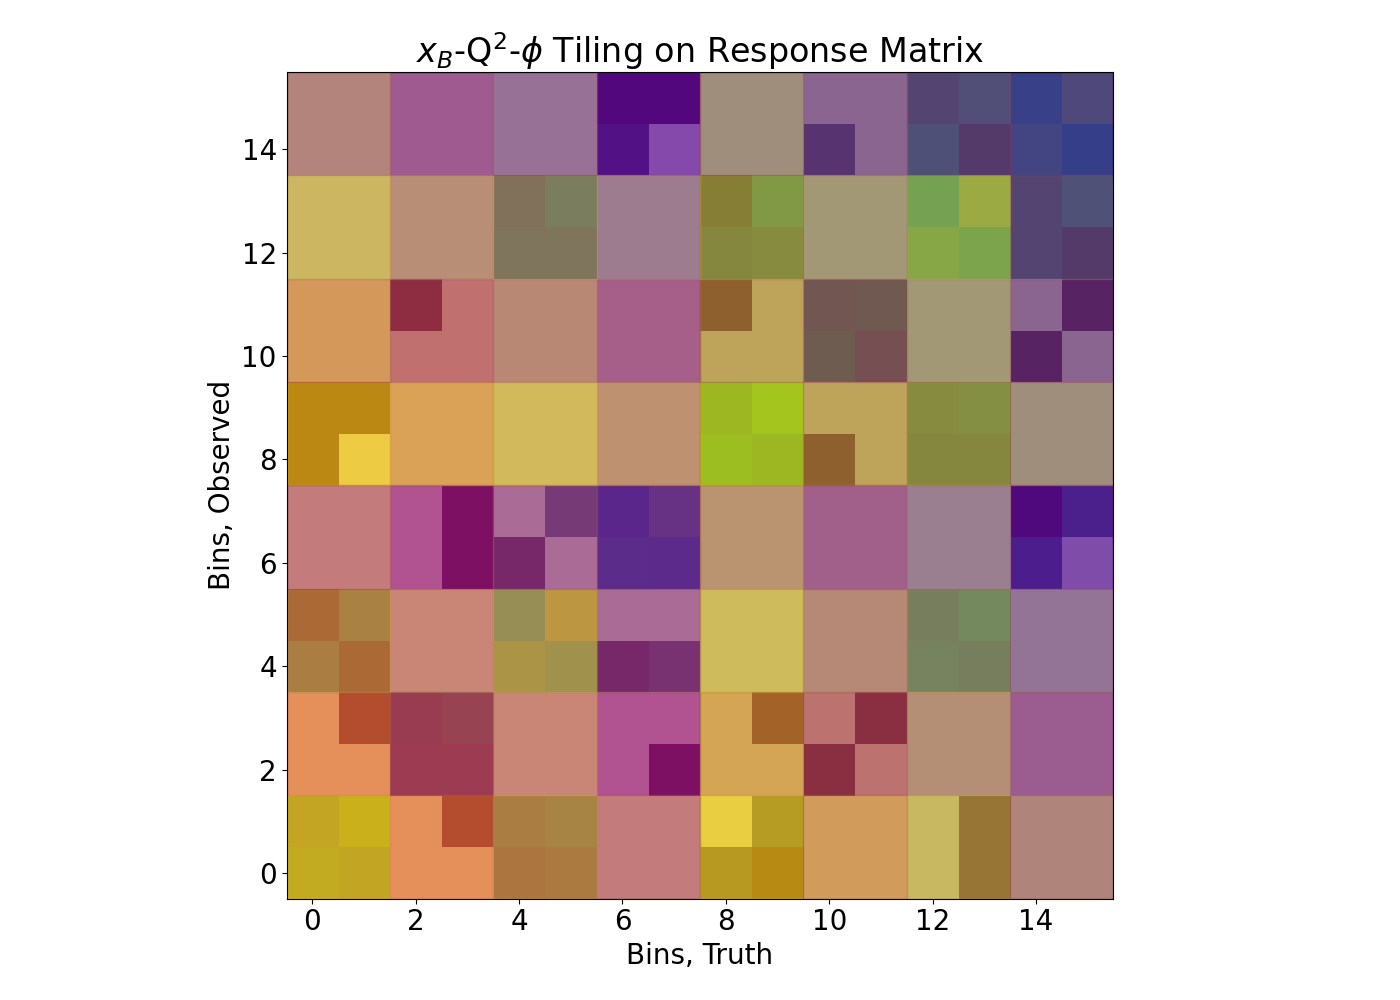
\includegraphics[width=0.45\textwidth]{Chapters/Ch5-Further/0_IBU/pics/4d-2n_example/plaid/4D_2bin_sample_response_matrix_xb_q2_phi.png}
        \label{fig:response_matrix_xb_q2_phi}}
        \hfill
        \subfloat[][4D 2-Bin Sample Response Matrix xb q2 phi t]{
        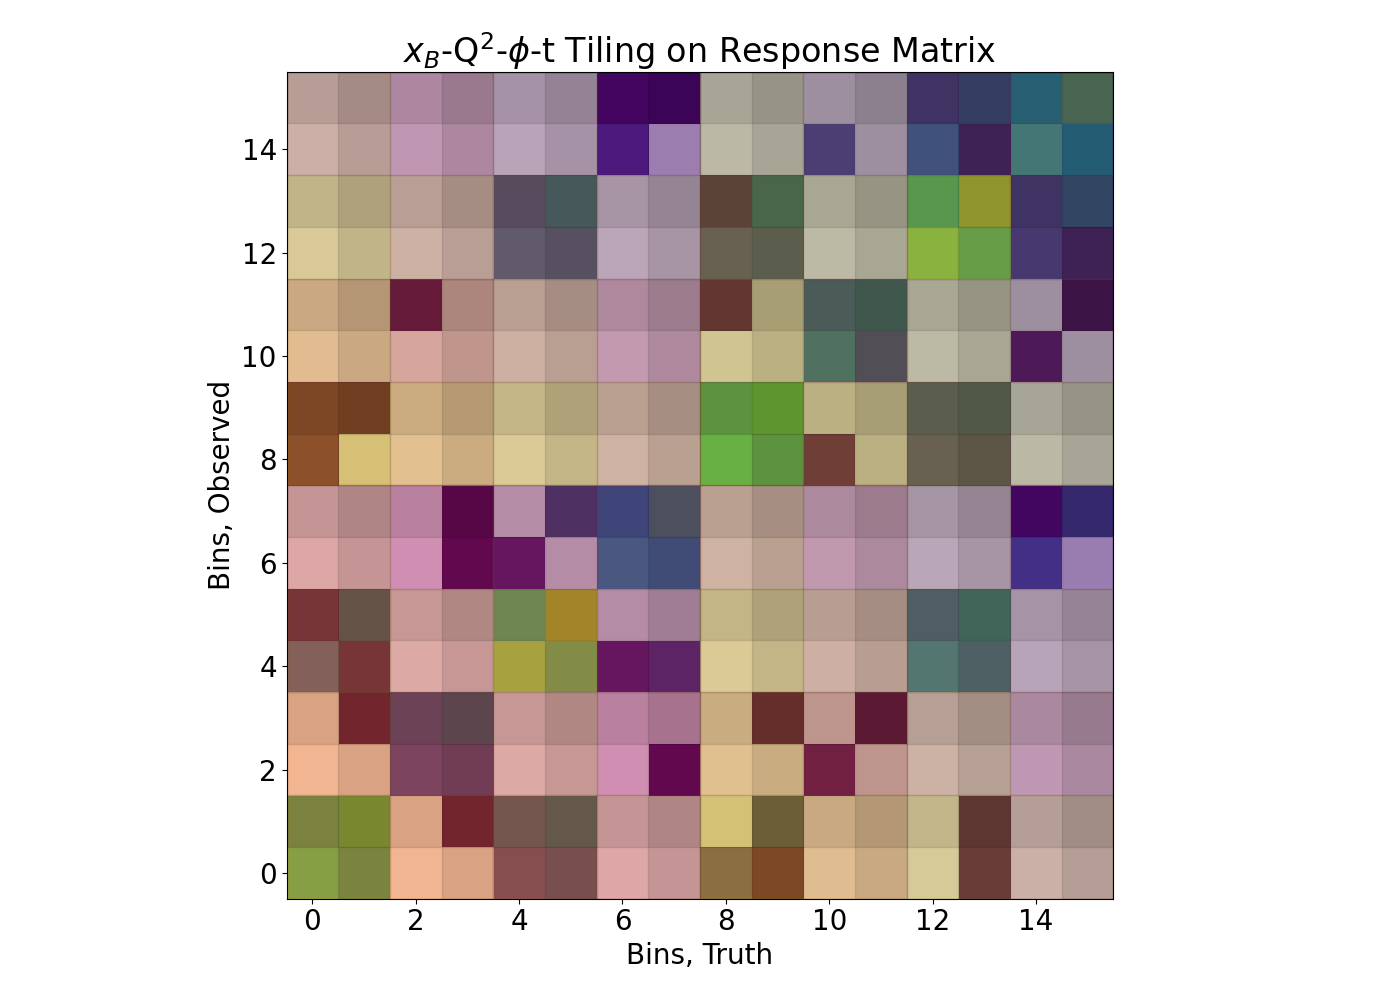
\includegraphics[width=0.45\textwidth]{Chapters/Ch5-Further/0_IBU/pics/4d-2n_example/plaid/4D_2bin_sample_response_matrix_xb_q2_phi_t.png}
        \label{fig:response_matrix_xb_q2_phi_t}}
        \caption{4D 2-Bin Sample Response Matrix}
        \label{fig:4D_2bin_sample_response_matrix}
    \end{figure}

        \begin{figure}[H]
        \centering
        \subfloat[xb vs q2]{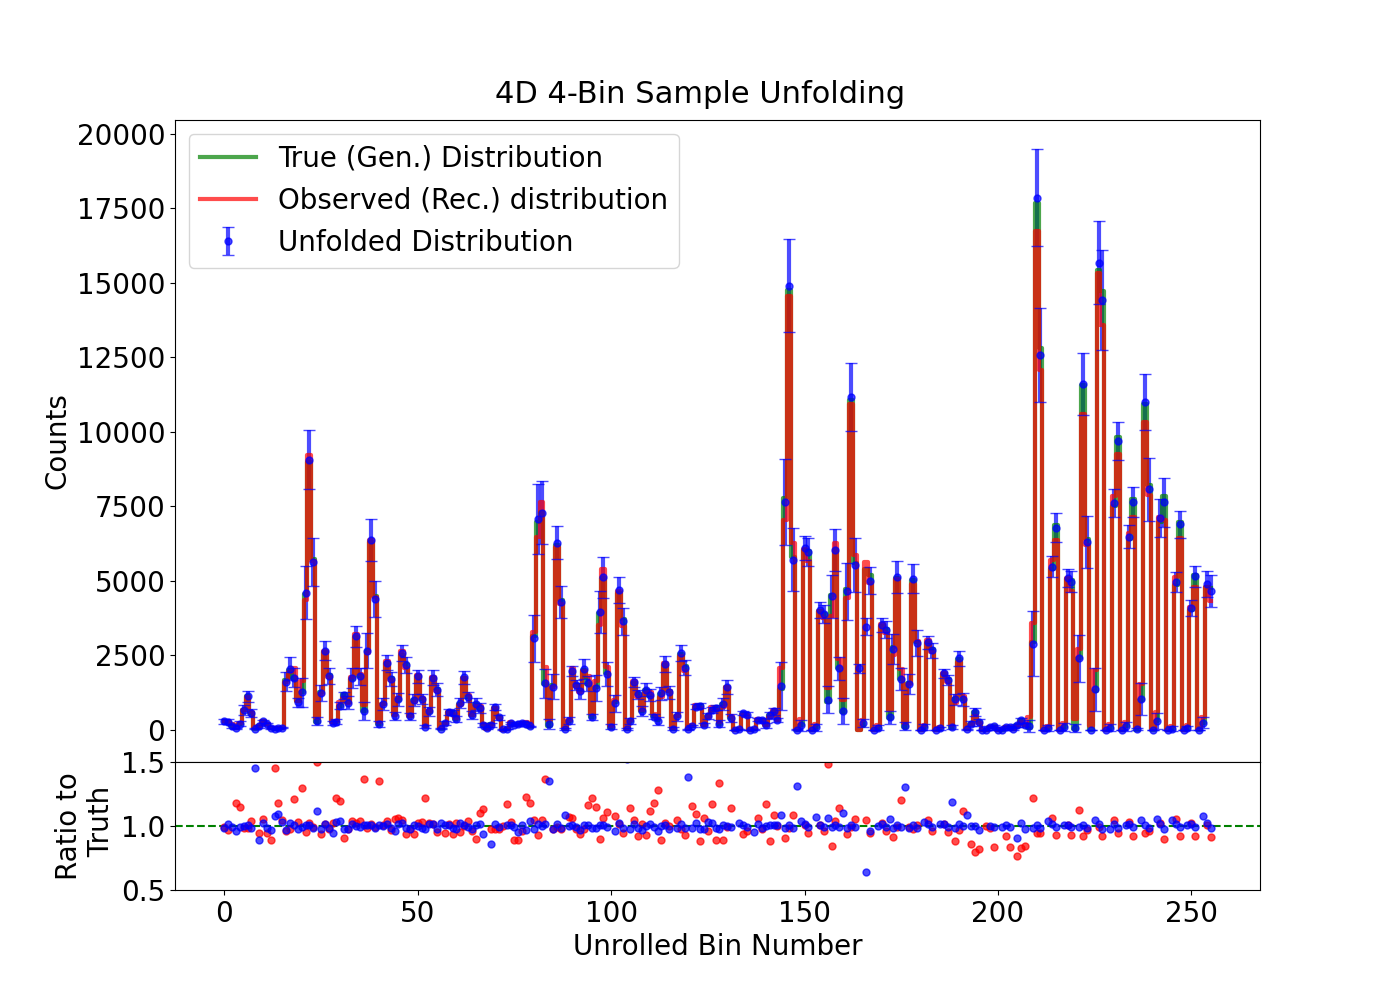
\includegraphics[trim={0 0 0 0},clip,width=0.5\textwidth]{Chapters/Ch5-Further/0_IBU/pics/4d-4n-3nkernel/4D_4bin_sample_unfolding.png}}
        \hfill
        \subfloat[phi vs t]{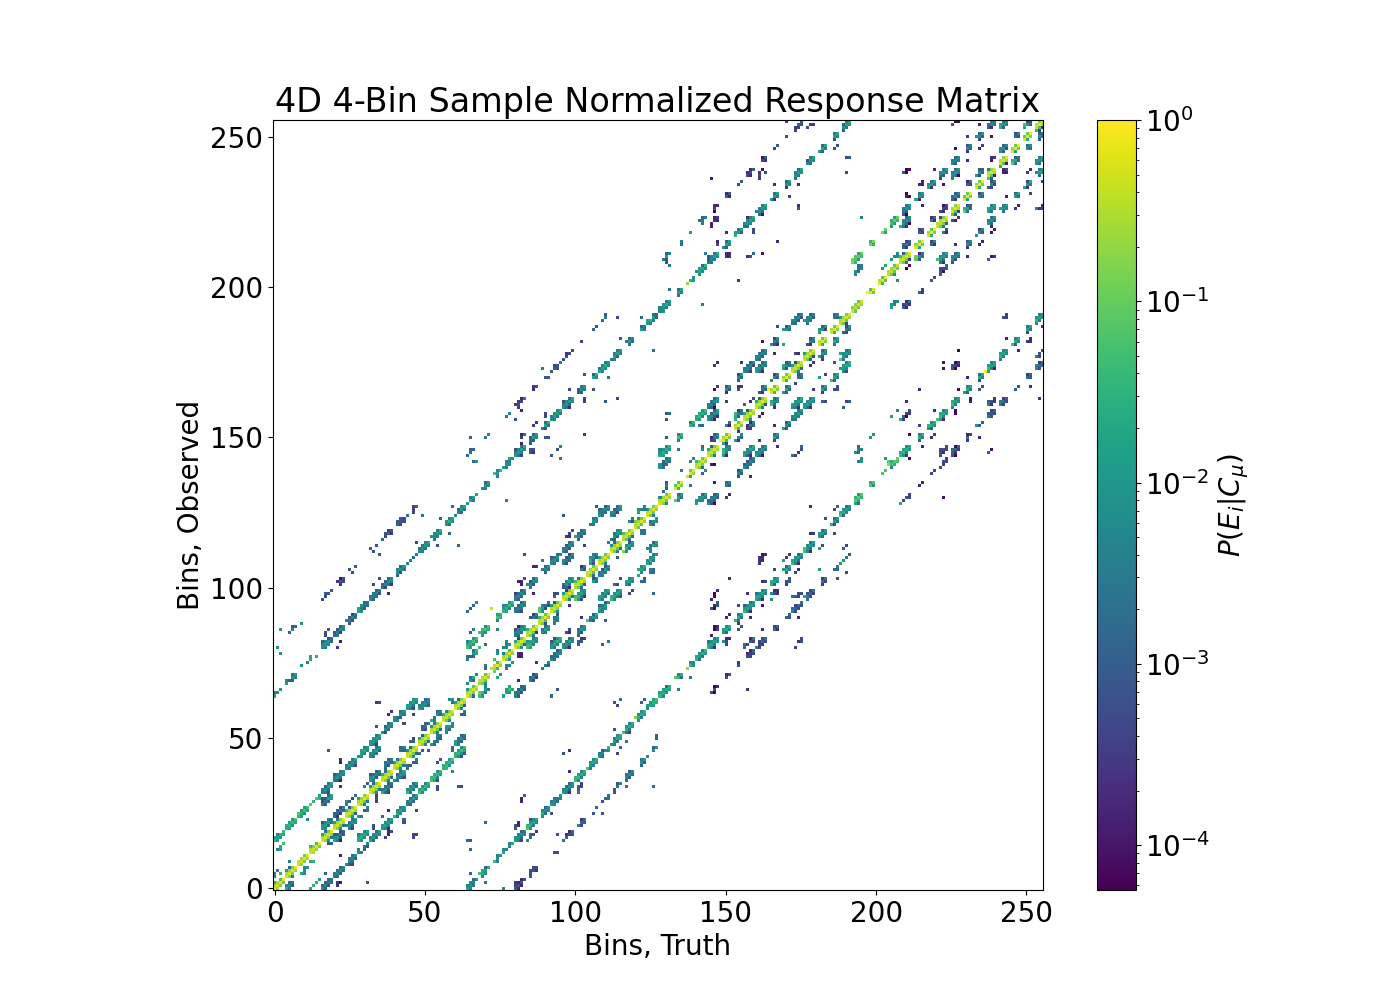
\includegraphics[trim={0 0 0 0},clip,width=0.5\textwidth]{Chapters/Ch5-Further/0_IBU/pics/4d-4n-3nkernel/4D_4bin_sample_normalized_response_matrix.png}}
        
        \caption[Binning]{Binning. }\label{fig:mig_ex}
    \end{figure}
    
    \iffalse
    Data scaling
    506 unrolled bins = 506x506 response matrix = 506x506x506x506 matrix = (256036, 256036) = 65554433296 entries with 8 bytes (float64) or 4 bytes (float32) data each, yielding 524435466368 (float64) / 1024\^3 = 488 GiB of memory needed (or 244 for float 32). 
    This means full matrix would have 8*10*8*10 = 6400 x 6400 response matrix =  6400 x 6400 x  6400 x 6400 cov matrix = 1.6777216e+15 entries = 12207.03125 TiB = 12.2 PiB memory
    “”” ON THE RID. SIZE OF MATRIX UNFOLDING:
    The error message you're seeing is a MemoryError from the NumPy package in Python. Specifically, the error message indicates that your Python program tried to allocate a substantial amount of memory for an array, but there was not enough available to satisfy the request. In this case, your script tried to allocate approximately 488 GiB (Gigabytes) of memory for an array of shape (256036, 256036) with data type float64.
    
    This memory error is coming from the multinomial\_covariance function within the PyUnfold package. The function attempts to create a covariance matrix (CovPP) of size (cbins * ebins) x (cbins * ebins). The specific line of code that leads to the error is:
    
    python
    Copy code
    CovPP = np.zeros((cbins * ebins, cbins * ebins))
    Given the error message, it seems cbins * ebins equals 256036, which means the function is trying to create a massive 256036 x 256036 matrix. Each float64 element requires 8 bytes, so the total memory required for this matrix is about 488 GiB. This is a very large amount of memory, and it seems your machine does not have sufficient memory to accommodate this request.
    
    To fix this error, you have several options:
    
    If possible, reduce the size of the arrays cbins and/or ebins.
    Use a machine with more memory if your task necessarily requires such large arrays.
    Modify your code to use a more memory-efficient approach, such as processing the data in smaller chunks or using a more memory-efficient data type if the precision of float64 is not required.
    If the algorithm allows, consider using sparse representations for the covariance matrix. Sparse representations only store non-zero elements and can be very memory-efficient for matrices with lots of zeros.
    
    \fi
    Data unfolding is a class of techniques used in high energy physics and other fields to estimate the true underlying distribution of a quantity from measured data that has been distorted by a measurement apparatus (cousins2012unfolding, kuhlen2011unfolding). Unfolding is crucial in situations where the measurement apparatus cannot be perfectly calibrated, or the response of the measurement apparatus cannot be accurately modeled.
    
    Unfolding techniques have been applied in various areas of experimental physics, such as in the estimation of the neutrino energy spectrum in neutrino oscillation experiments (abe2010indication), and in measurements of the top quark mass in collider experiments (chatrchyan2013measurement). These techniques allow researchers to correct for distortions and biases in the measured data, and to recover the true underlying distributions of the quantities of interest.
    
\clearpage
\section{Unfolding Methods}


\clearpage
\section{Iterative Bayesian Unfolding}
    
    Iterative Bayesian Unfolding (IBU) is a specific unfolding technique that uses Bayesian probability to account for the statistical uncertainty in the unfolding process (agostini1995bayesian, blobel2002unfolding). This technique constructs a probability model of the response of the measurement apparatus, and iteratively refines an estimate of the true underlying distribution by conditioning on the measured data.
    
    IBU starts with an initial estimate of the true distribution, and in each iteration, it modifies this estimate based on the residuals between the measured data and the data predicted by the current estimate. The iterations continue until the estimate converges to a stable solution. One of the key advantages of IBU is that it naturally incorporates uncertainties due to statistical fluctuations in the measured data, and it provides a measure of uncertainty for the unfolded distribution.
    
    When comparing unfolding techniques, it is important to consider the strengths and weaknesses of each approach. Iterative Bayesian Unfolding (IBU) has the advantage of being able to handle a non-linear relationship between the measured and true distributions, and can incorporate prior knowledge about the response matrix. However, it has the potential to overfit data and the result can be sensitive to the choice of the prior. Tikhonov Regularization, also known as Ridge Regression, has the advantage of being simple to implement and more robust to noise in the response matrix, but can suffer from a high bias if the regularization parameter is not chosen carefully. Lastly, Singular Value Decomposition (SVD) has the advantage of dealing well with ill-posed problems and being computationally efficient, but it assumes linearity and can be sensitive to small changes in the response matrix, which may introduce instability. Thus, the selection between these techniques should be guided by the nature of the data, the noise in the measurements, and the complexity of the response matrix~(hoaglin2003understanding,cowan1998statistical,dAgostini:1994fjg,svd).
    
    \begin{enumerate}
        \item \textbf{Initialization:} Start with an initial estimate of the true distribution, often taken to be the measured distribution. This is known as the prior.
    
        \item \textbf{Calculation of the expected measured distribution:} Using the response matrix and the current estimate of the true distribution, calculate the expected measured distribution. The response matrix describes the probability that an event in a given true bin is observed in each of the observed bins.
    
        \item \textbf{Update of the prior:} Update the estimate of the true distribution by applying Bayes' theorem. This involves multiplying the current prior by the ratio of the actual measured distribution to the expected measured distribution calculated in the previous step. This updated distribution serves as the new prior for the next iteration.
    
        \item \textbf{Normalization:} Normalize the updated distribution so that the total number of events is conserved.
    
        \item \textbf{Iteration:} Repeat steps 2-4 until the changes in the estimated true distribution from iteration to iteration become small, indicating that the algorithm has converged.
    \end{enumerate}
    
    This method can be further enhanced by introducing regularization to avoid potential instabilities and overfitting issues. The choice of the initial prior, the stopping criterion for the iterations, and the form of the regularization can have a significant impact on the unfolding results~\cite{dagostini1995probability}.
    
    
    \begin{figure}[ht]
    \centering
    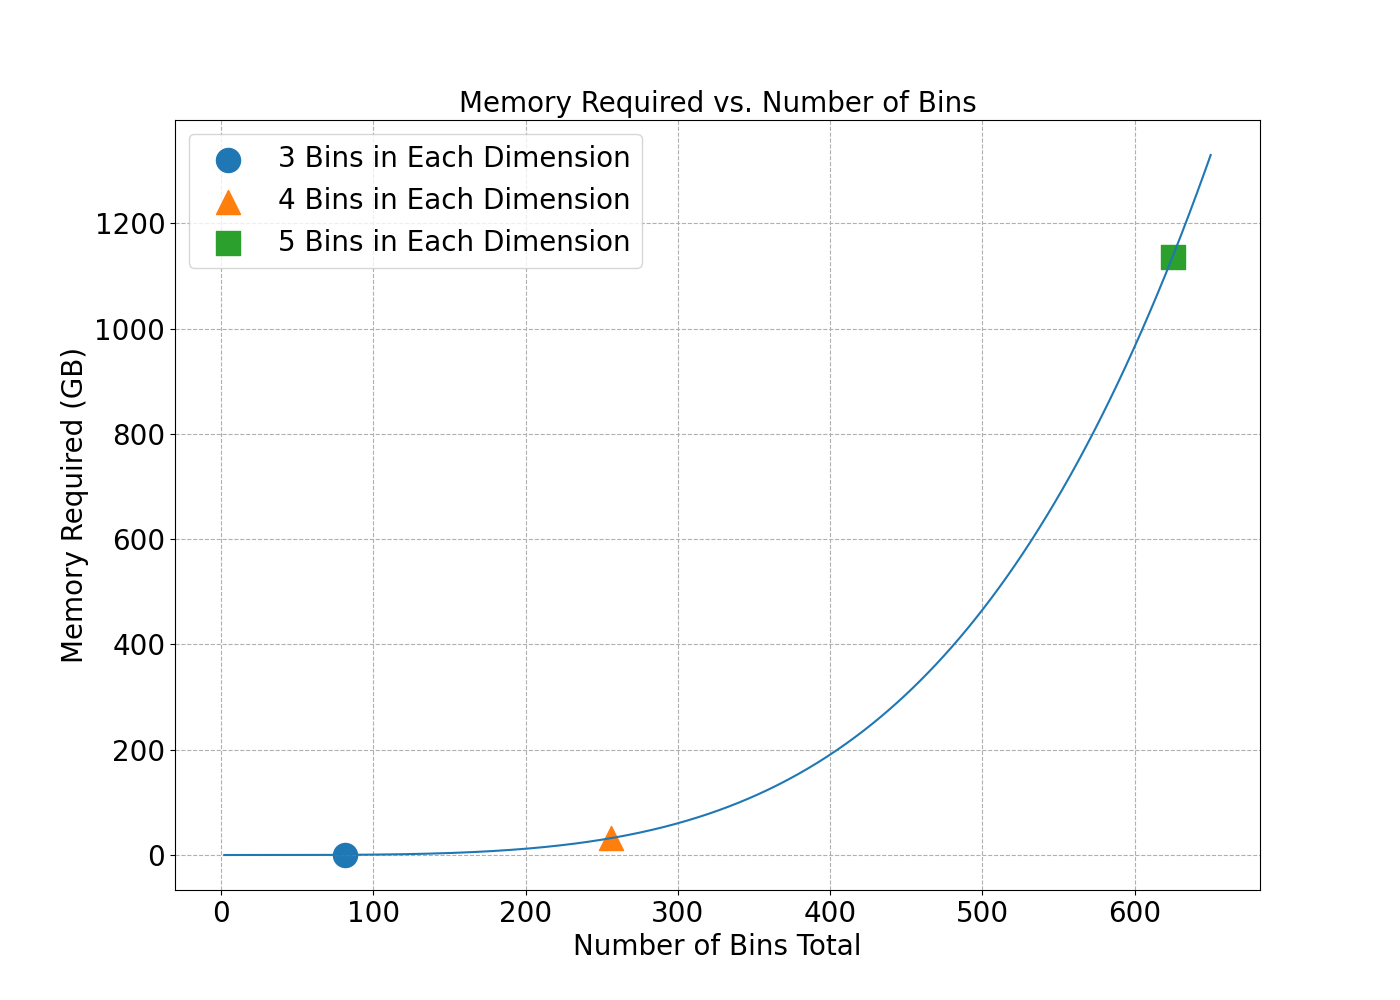
\includegraphics[trim={0 0 0 0},clip,width=\textwidth]{Chapters/Ch5-Further/0_IBU/pics/memory_required_vs_number_of_bins_in_each_dim.png}
    \caption[words]{words}
    \label{fig:ibu10}
    \end{figure}
    
    \iffalse
    Agostini, G. (1995). "A multidimensional unfolding method based on Bayes' theorem". Nucl. Instrum. Methods Phys. Res. A 362, 487–498. DOI: 10.1016/0168-9002(95)00274-X
    Blobel, V. (2002). "Unfolding methods in high-energy physics experiments". DOI: 10.5170/CERN-1984-009.171.
    Cousins, R.D. (2012). "Lecture Notes on Statistics for Physicists". arXiv preprint arXiv:1205.2634.
    Kuhlen, M., Pato, M., & Strigari, L. E. (2011). "Direct Detection of Dark Matter Annual Modulation in Simplified Models". Phys. Rev. D, 84, 12. DOI: 10.1103/PhysRevD.84.123005.
    Abe, K. et al. (2010). "Indication of Electron Neutrino Appearance from an Accelerator-produced Off-axis Muon Neutrino Beam". Phys. Rev. Lett., 107, 041801. DOI: 10.1103/PhysRevLett.107.041801.
    Chatrchyan, S. et al. (2013). "Measurement of the top-quark mass in all-jets $t\bar{t}$ events in pp collisions at $\sqrt{s}=7$ TeV". Eur. Phys. J. C, 73, 2494. DOI: 10.1140/epjc/s10052-013-2494-4.
    \fi
    
    Here we talk about Iterative Bayesian unfolding to not have bin migration issues
    
    Notes on Omnifold from Anselm Vossen:
    I find this reference paper - \href{https://arxiv.org/pdf/1911.09107.pdf}{arxiv}.
    
    
    Bin migration issues grow with the number of binning dimensions - an analysis that has 80\% bin purity in each of four dimensions yields a 4D bin that has a purity of only 0.8$^4$=41\%. 
    
    
    The bin purity $P_{i}$ and bin efficiency $E_{i}$ are often used to measure the performance of a binning process. 
    
    The \textbf{bin purity} in bin $i$, denoted $P_{i}$, is defined as the fraction of the total amount in bin $i$ that actually belongs to bin $i$. Mathematically, this can be written as:
    
    \begin{equation}
    P_{i} = \frac{T_{ii}}{\sum_{j} T_{ij}}
    \end{equation}
    
    where $T_{ij}$ is the amount that originated in bin $j$ and ended up in bin $i$.
    
    The \textbf{bin efficiency} in bin $i$, denoted $E_{i}$, on the other hand, is the fraction of the total amount that originated in bin $i$ that ends up in bin $i$. This can be written as:
    
    \begin{equation}
    E_{i} = \frac{T_{ii}}{\sum_{j} T_{ji}}
    \end{equation}
    
    
    Bin migrations refer to the movement of data from one bin to another during a process of interest. For a process with $n$ bins, we can represent the bin migrations using an $n \times n$ matrix $T$, where each element $T_{ij}$ represents the amount that originated in bin $j$ and ended up in bin $i$. 
    
        
   
    
    
    
    Yes, that is the reference. You saw that I also posted a reference to the Hera analysis. I don’t think many others have used omnifold yet, since it is quite computationally intensive etc.
    My understanding is that Ben Nachman developed this and there has been follow up work by his group (if you just put his name into inspire you’ll see). E.g. I saw presentations on how to present the data. Here is a talk by Ben at a Jet workshop in 2021: \href{https://indico.bnl.gov/event/10555/contributions/54721/attachments/37368/61570/H1Measurement_EICWorkshopSeptember2021.pdf}{this paper}
     Miguel Arratia, who is also in CLAS collaborated on the H1 results. You could ask him for practical advice,
    
    From CHATGPT:
    
    
    Iterative Bayesian unfolding is a statistical technique used in particle physics and other fields to correct for detector effects and reconstruct the true distribution of a measured quantity.
    
    When particles are measured by a detector, the measurements can be distorted by various effects such as inefficiencies, energy loss, and detector resolution. This leads to a measured distribution that can be quite different from the true distribution.
    
    Unfolding techniques aim to invert these detector effects to estimate the true distribution from the measured one. The unfolding problem is challenging because it is ill-posed; small fluctuations in the data can lead to large fluctuations in the unfolded result.
    
    Bayesian unfolding is based on Bayes' theorem and uses a prior probability distribution that reflects our knowledge (or assumptions) about the true distribution before the measurement. The Bayesian approach allows for the incorporation of systematic uncertainties into the unfolding process.
    
    Iterative Bayesian unfolding is a variant of Bayesian unfolding that iteratively applies the unfolding procedure. The output of one iteration is used as the prior for the next iteration. This iteration process is repeated until the result converges.
    
    Please note that unfolding techniques are sensitive to the chosen model and prior, and they require careful validation and error estimation. The choice between iterative Bayesian unfolding and other unfolding techniques (like matrix inversion or regularized unfolding) often depends on the specific problem and the constraints of the analysis.

\section{Method of Implementation}
    81 x 81 (unrolled) bins
    
        \begin{figure}[ht]
        \centering
        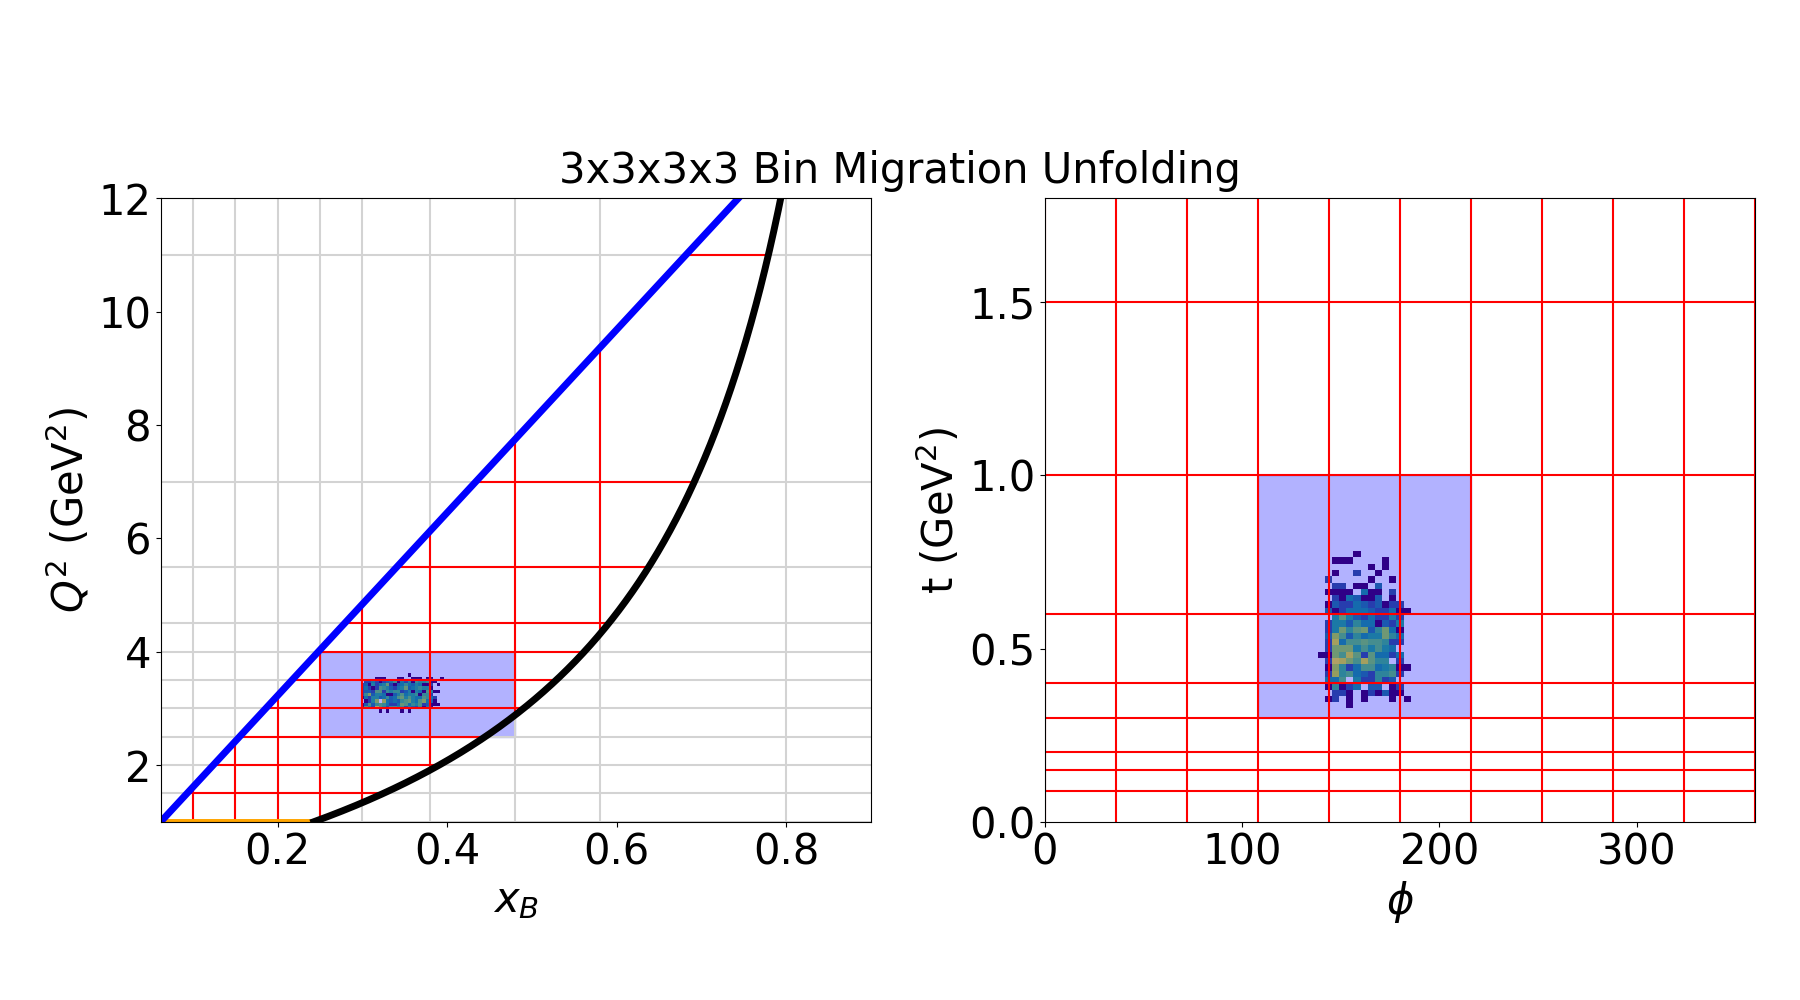
\includegraphics[trim={0 0 0 0},clip,width=\textwidth]{Chapters/Ch5-Further/0_IBU/pics/kerneling/bin_migration_1_1_1_1.png}
        \caption[words]{words}
        \label{fig:ibu1}
        \end{figure}
    
    
    \begin{figure}[ht]
    \centering
    \subfloat[][]{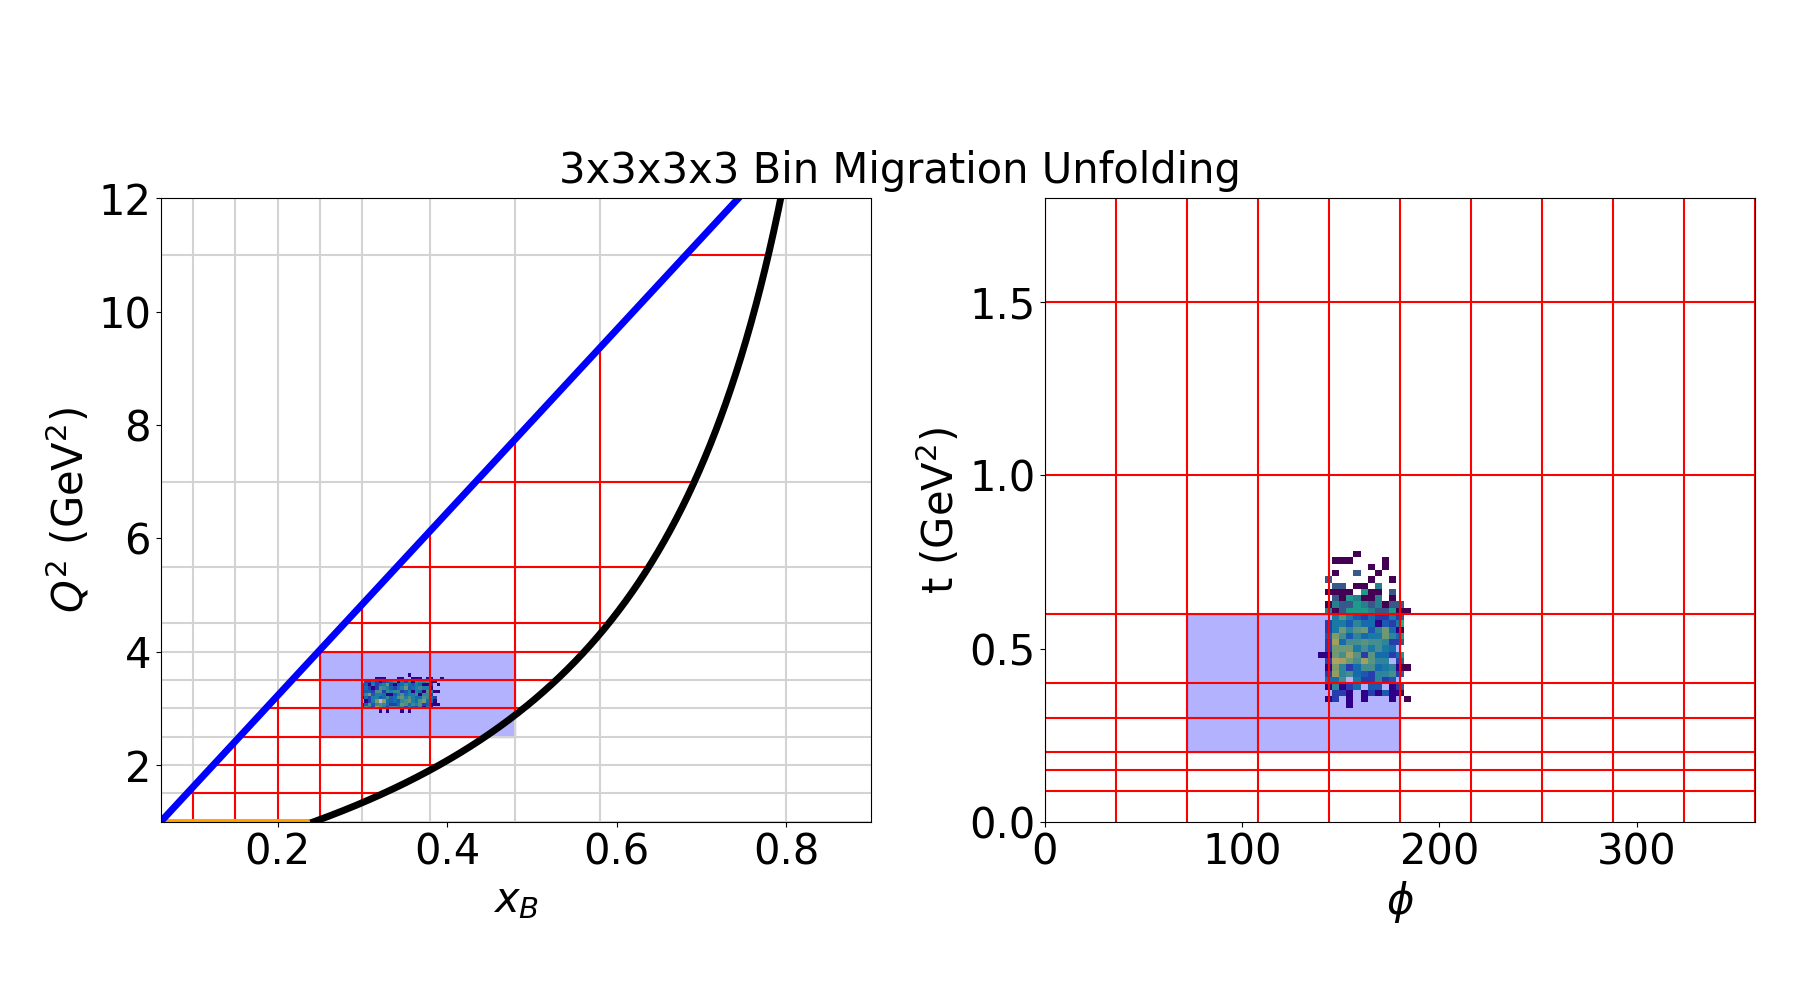
\includegraphics[trim={22.5cm 0 0 5cm},clip,width=0.3\textwidth]{Chapters/Ch5-Further/0_IBU/pics/kerneling/bin_migration_1_1_2_2.png}}
    \subfloat[][]{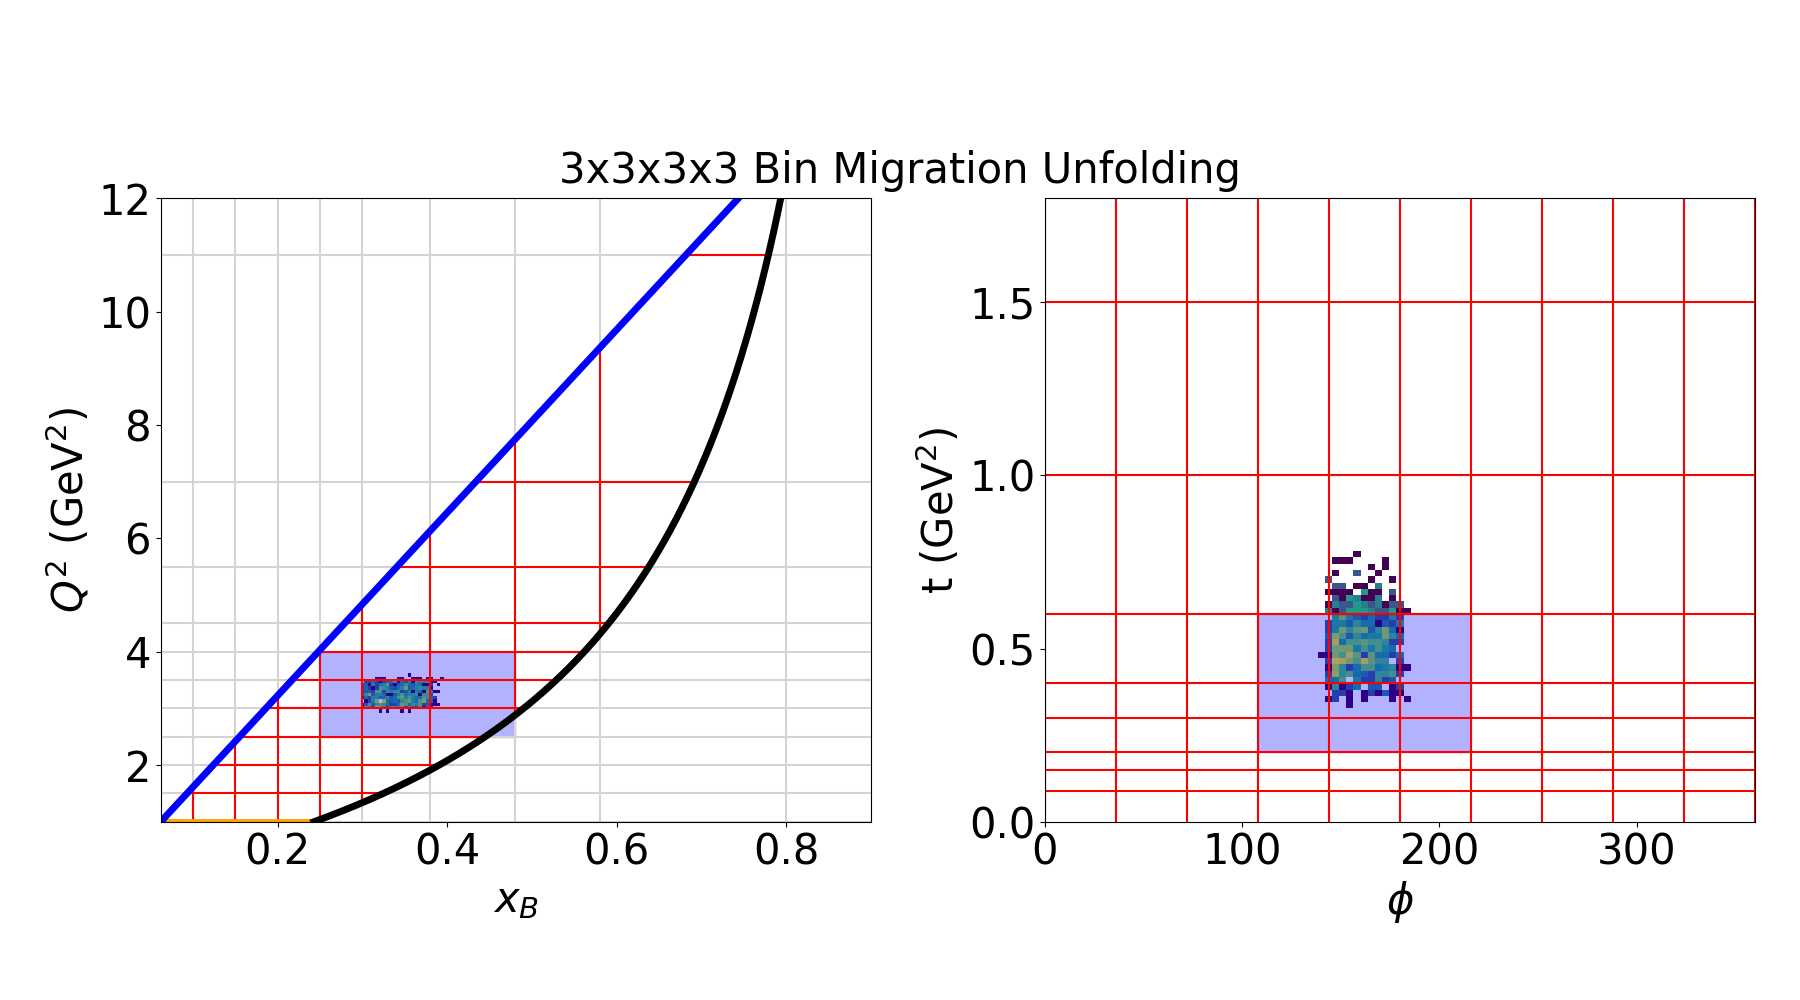
\includegraphics[trim={22.5cm 0 0 5cm},clip,width=0.3\textwidth]{Chapters/Ch5-Further/0_IBU/pics/kerneling/bin_migration_1_1_2_1.png}}
    \subfloat[][]{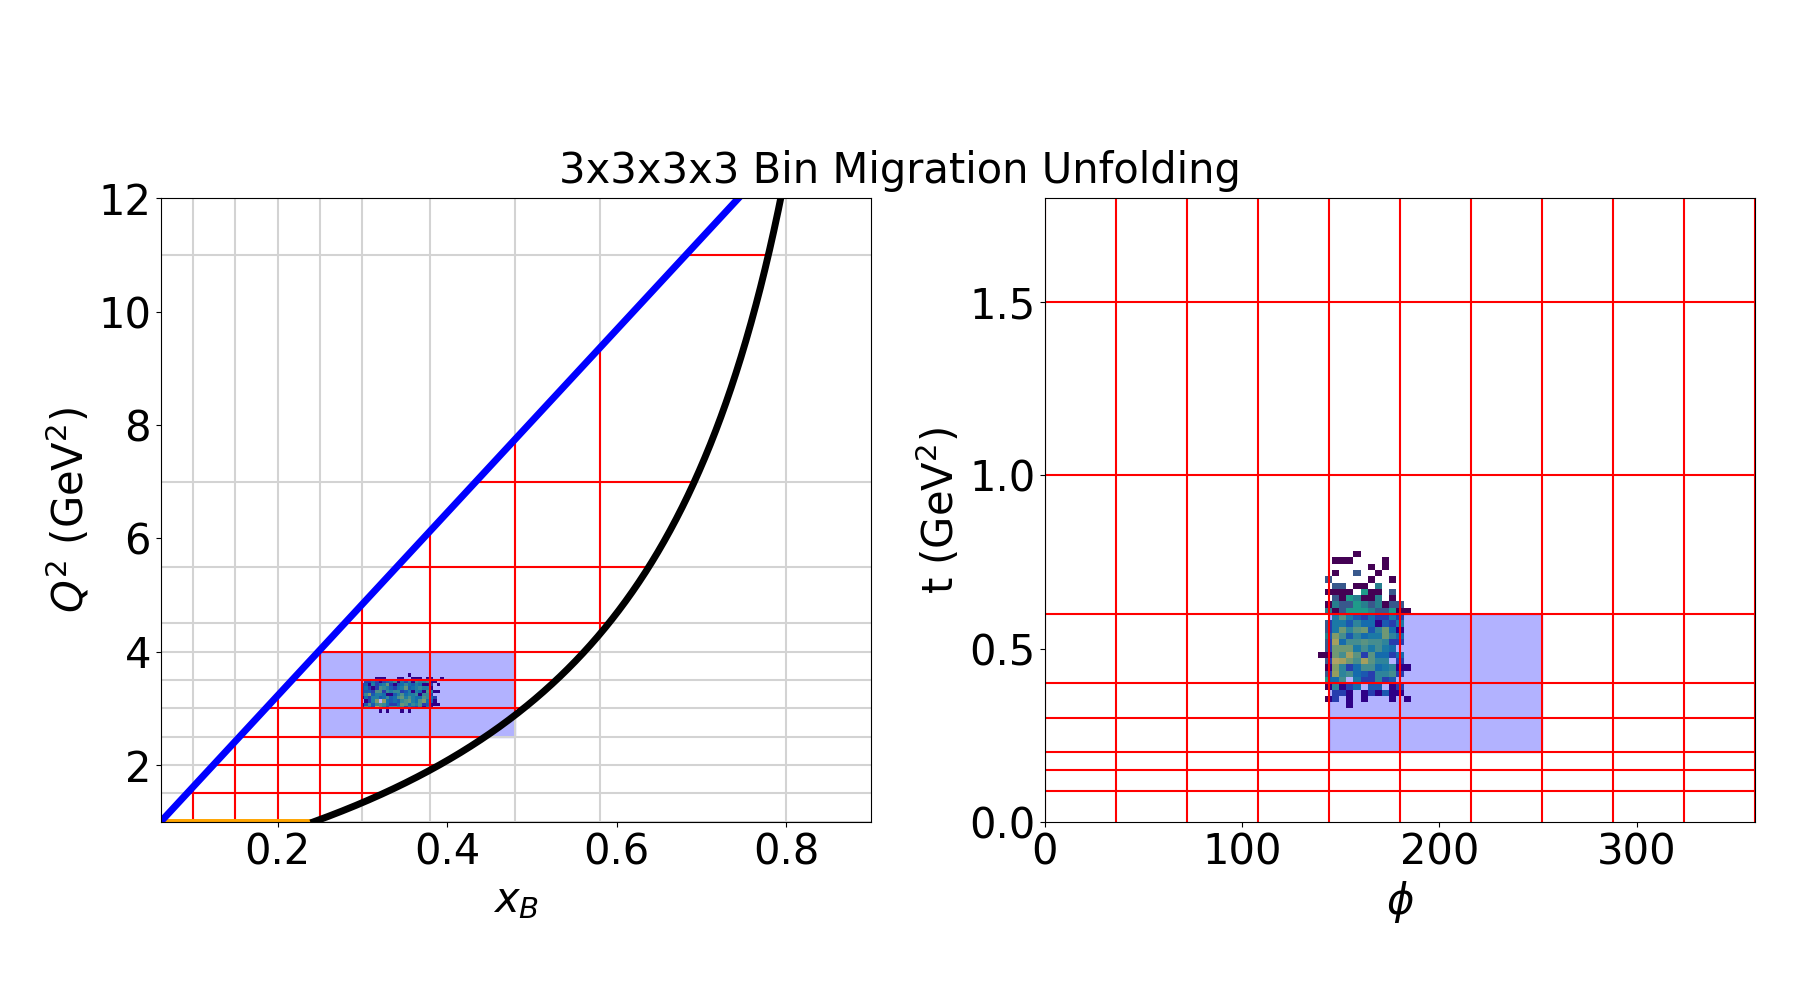
\includegraphics[trim={22.5cm 0 0 5cm},clip,width=0.3\textwidth]{Chapters/Ch5-Further/0_IBU/pics/kerneling/bin_migration_1_1_2_0.png}}\\
    \subfloat[][]{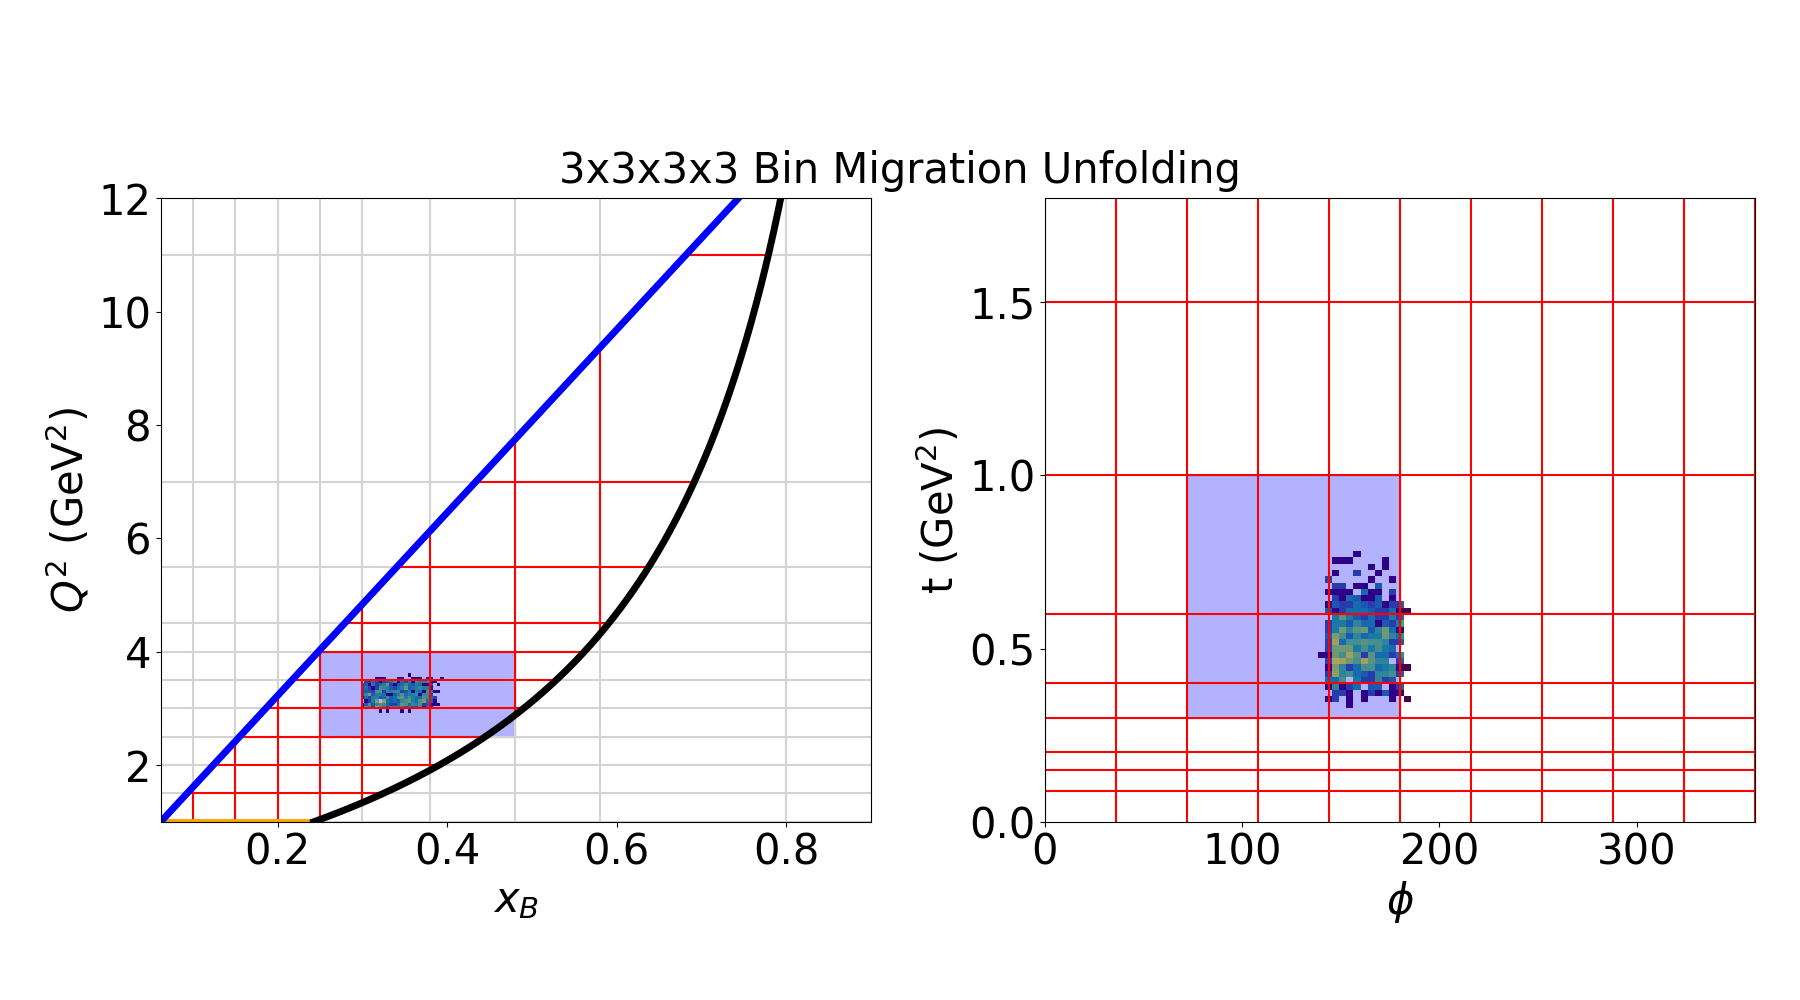
\includegraphics[trim={22.5cm 0 0 5cm},clip,width=0.3\textwidth]{Chapters/Ch5-Further/0_IBU/pics/kerneling/bin_migration_1_1_1_2.png}}
    \subfloat[][]{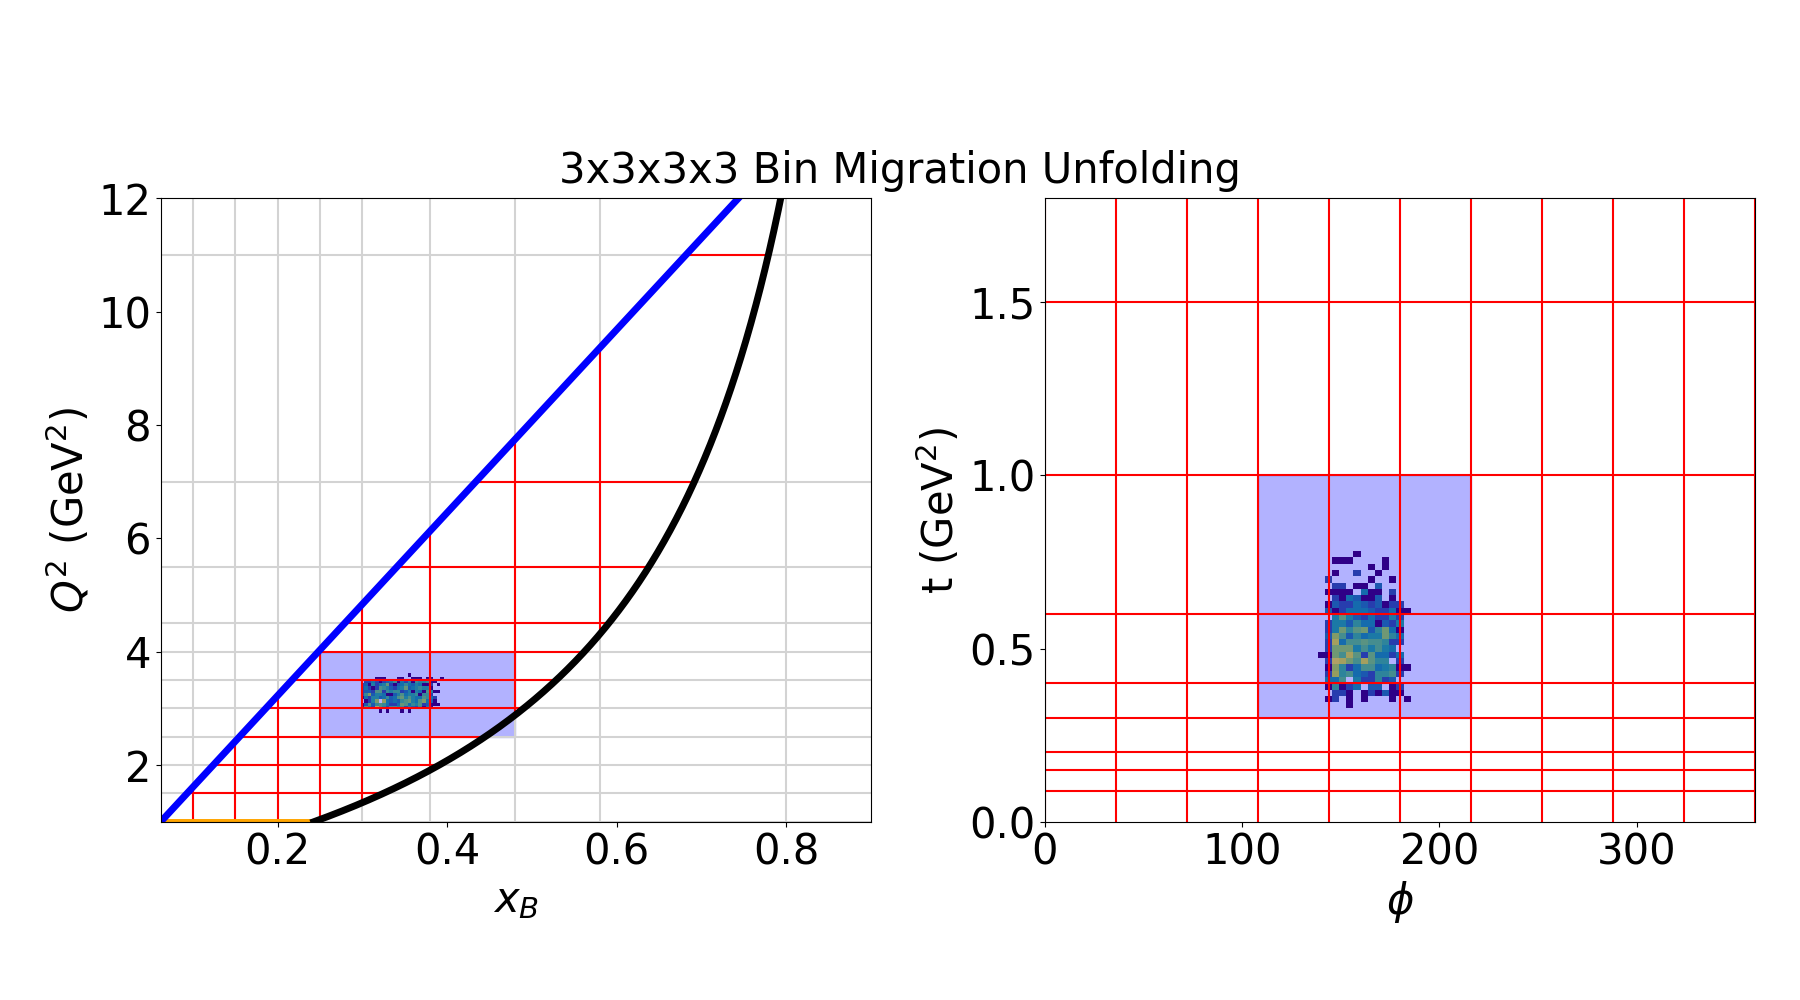
\includegraphics[trim={22.5cm 0 0 5cm},clip,width=0.3\textwidth]{Chapters/Ch5-Further/0_IBU/pics/kerneling/bin_migration_1_1_1_1.png}}
    \subfloat[][]{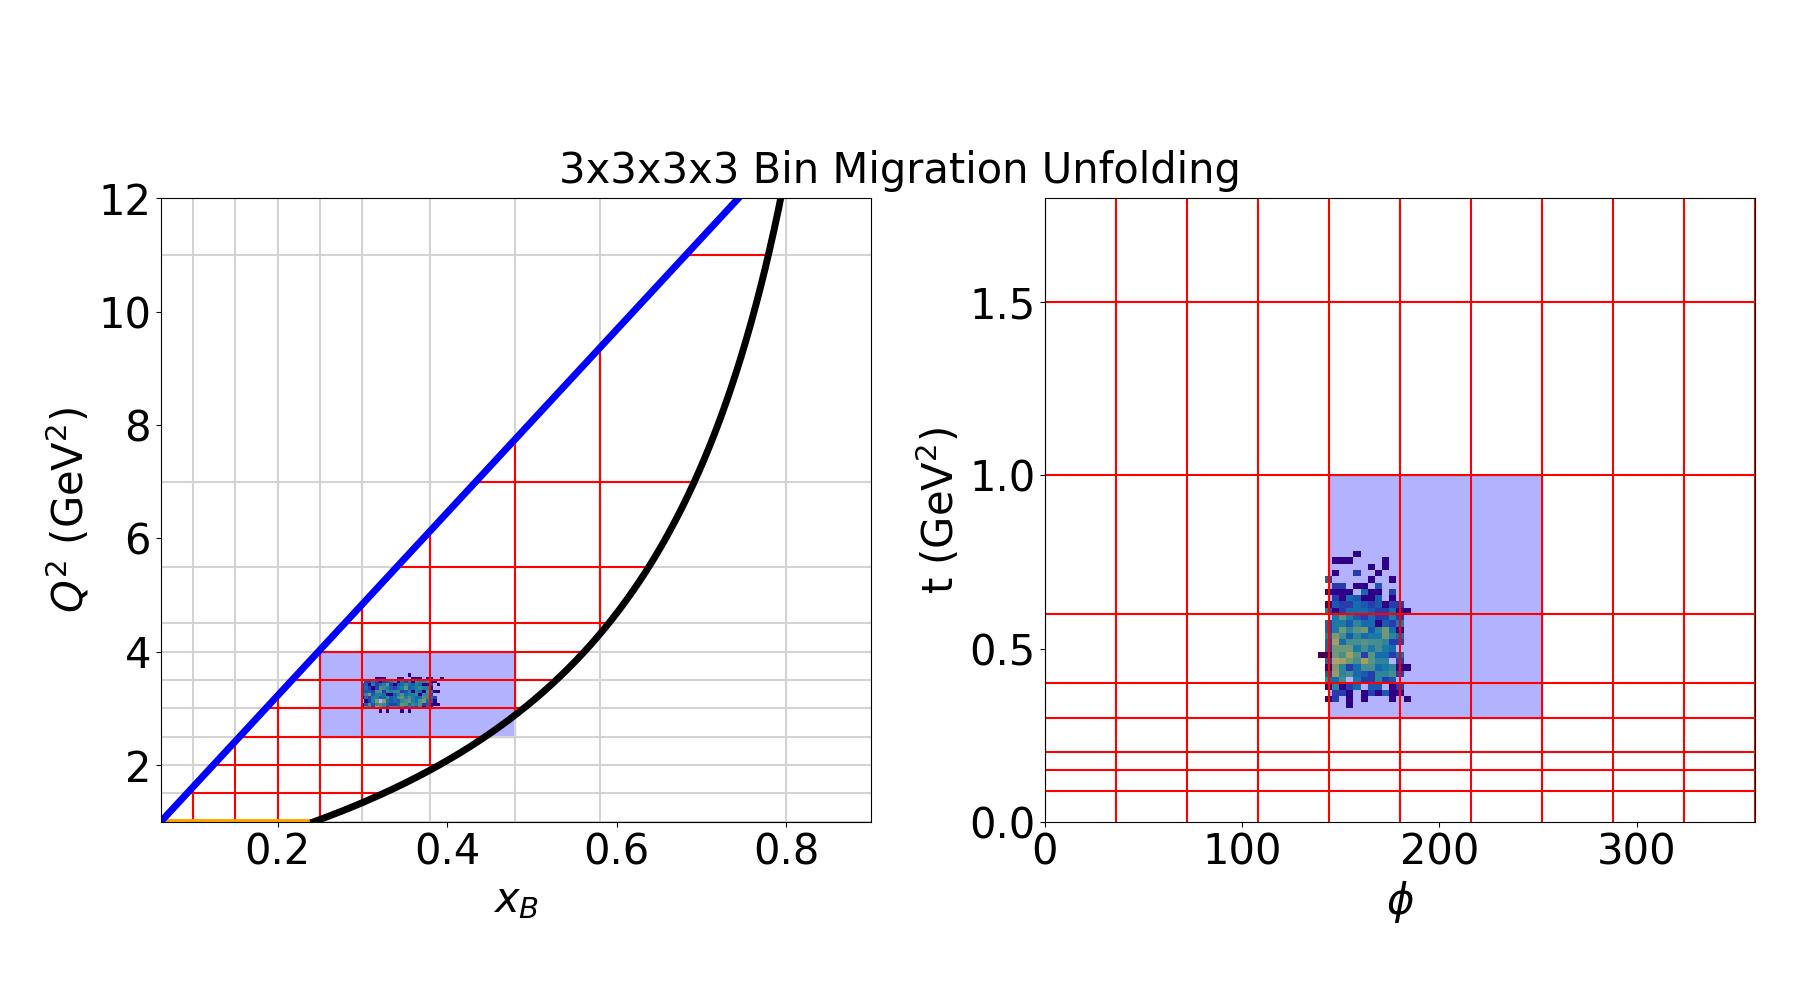
\includegraphics[trim={22.5cm 0 0 5cm},clip,width=0.3\textwidth]{Chapters/Ch5-Further/0_IBU/pics/kerneling/bin_migration_1_1_1_0.png}}\\
    \subfloat[][]{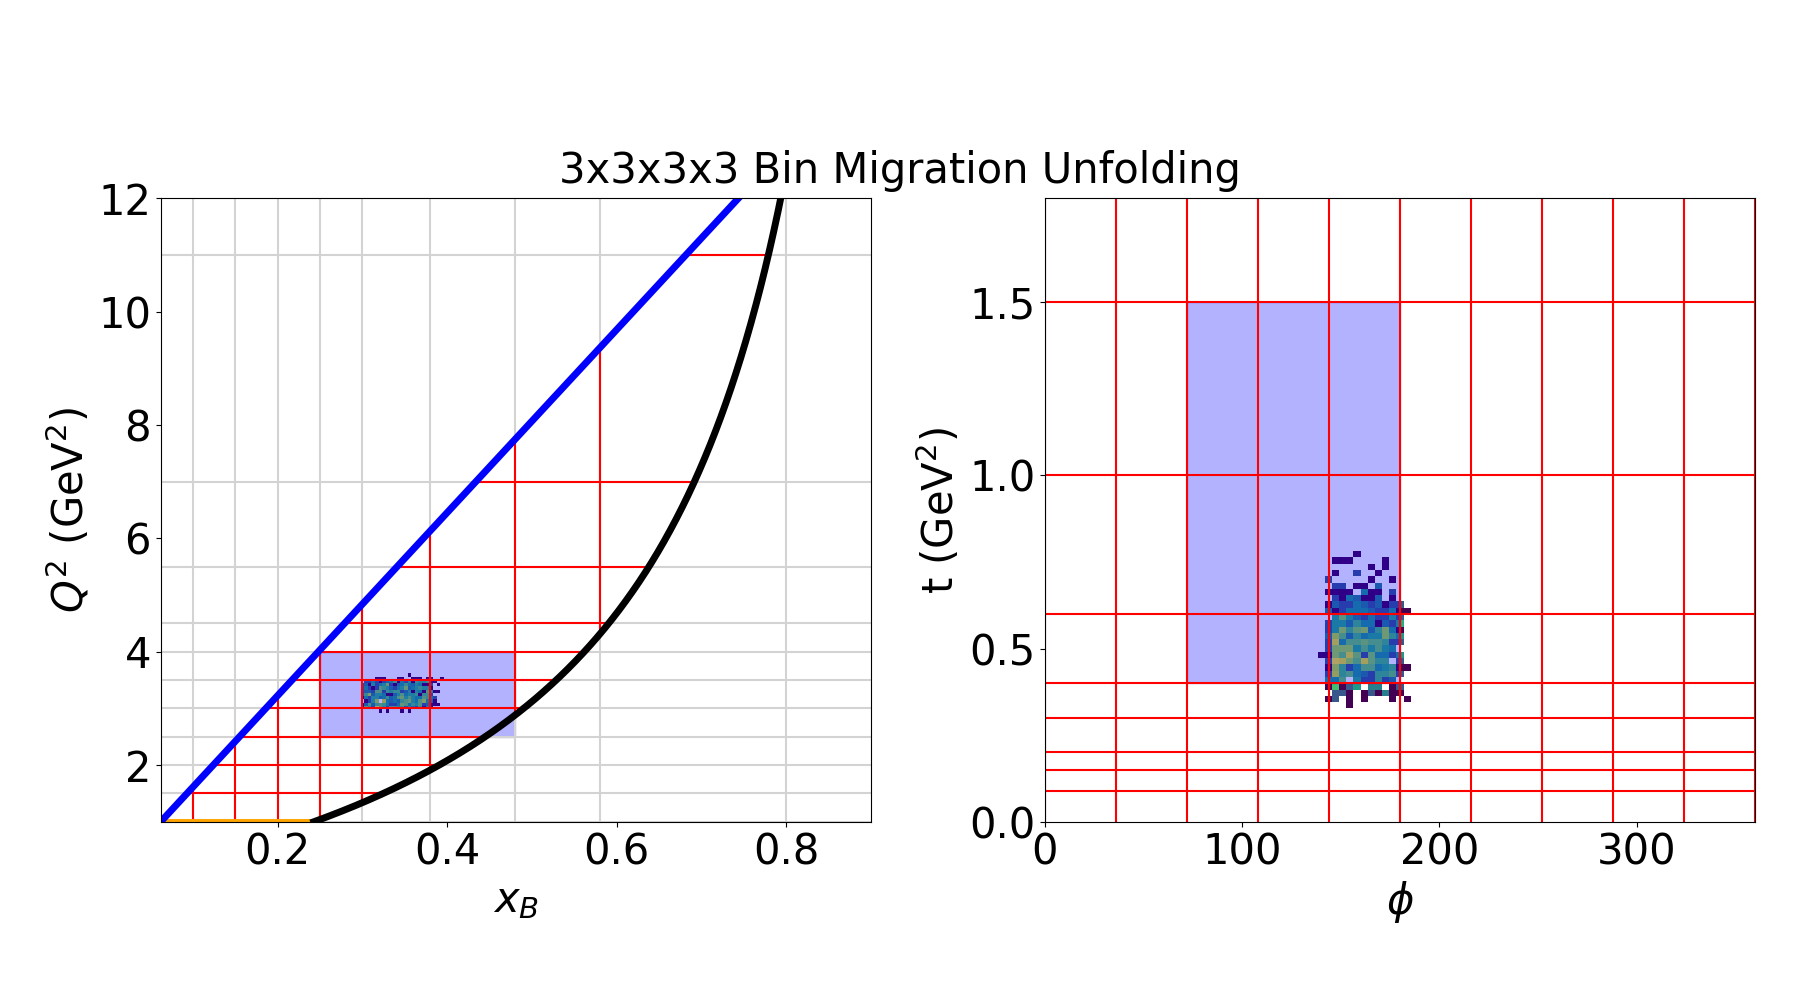
\includegraphics[trim={22.5cm 0 0 5cm},clip,width=0.3\textwidth]{Chapters/Ch5-Further/0_IBU/pics/kerneling/bin_migration_1_1_0_2.png}}
    \subfloat[][]{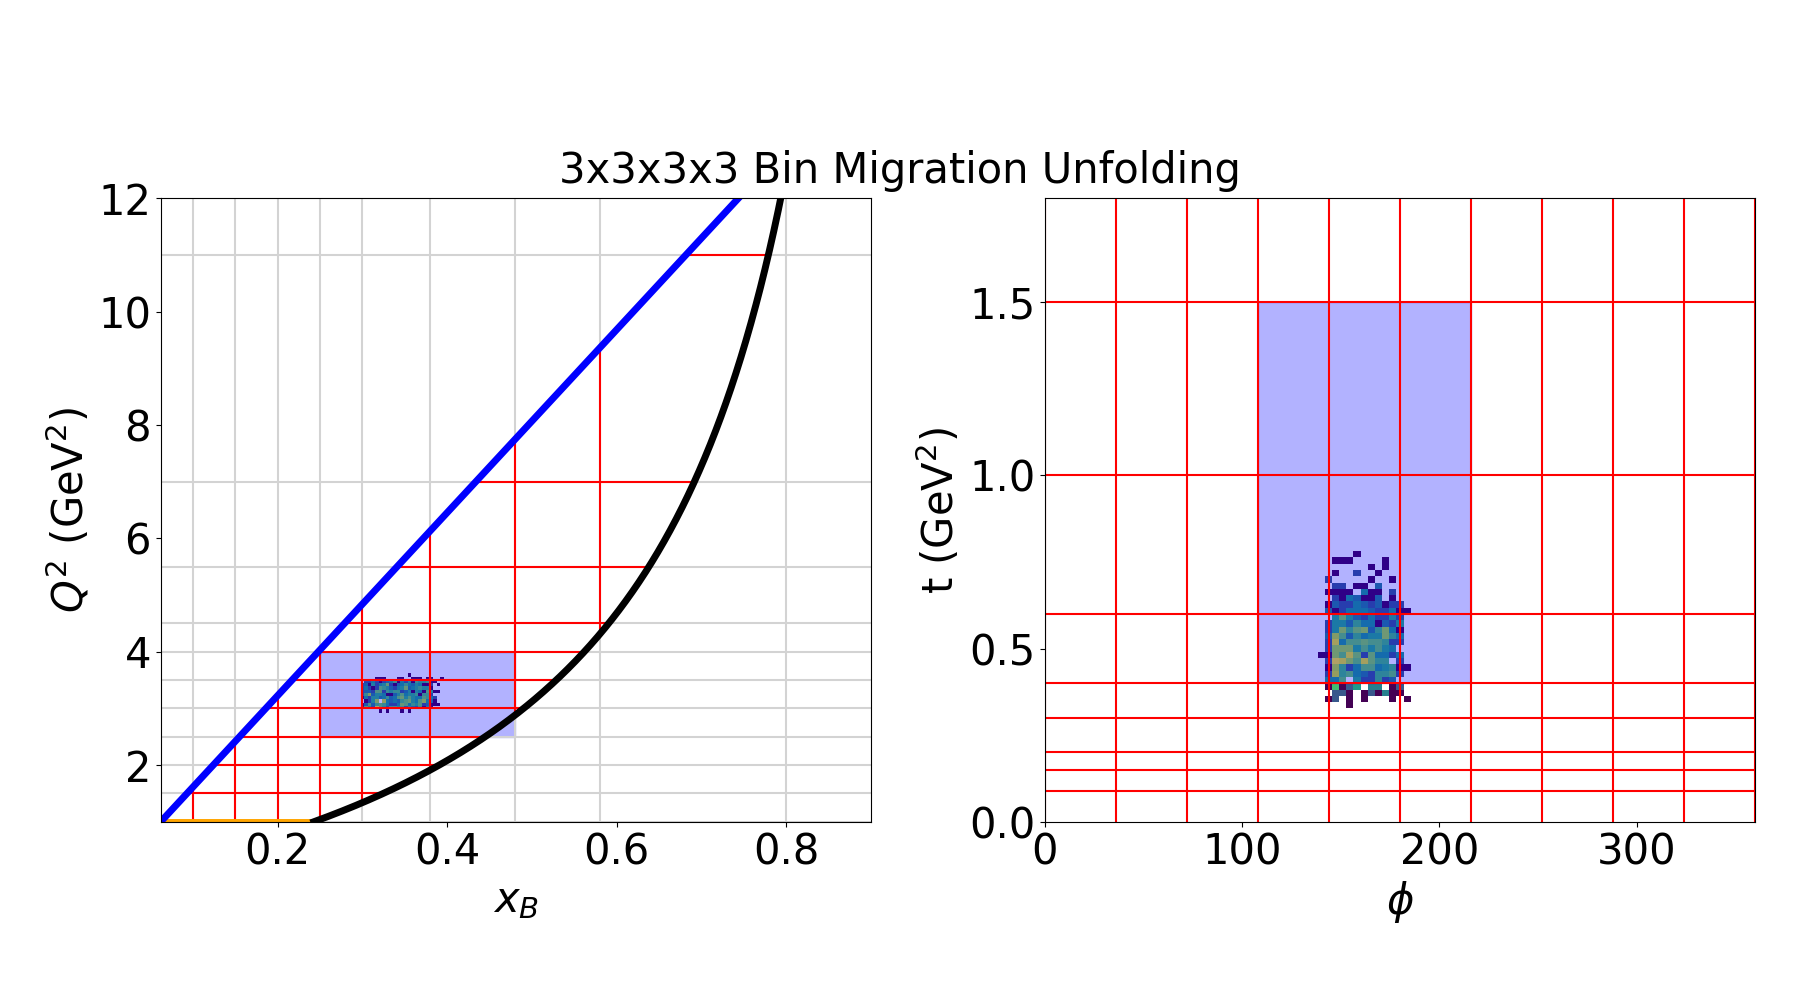
\includegraphics[trim={22.5cm 0 0 5cm},clip,width=0.3\textwidth]{Chapters/Ch5-Further/0_IBU/pics/kerneling/bin_migration_1_1_0_1.png}}
    \subfloat[][]{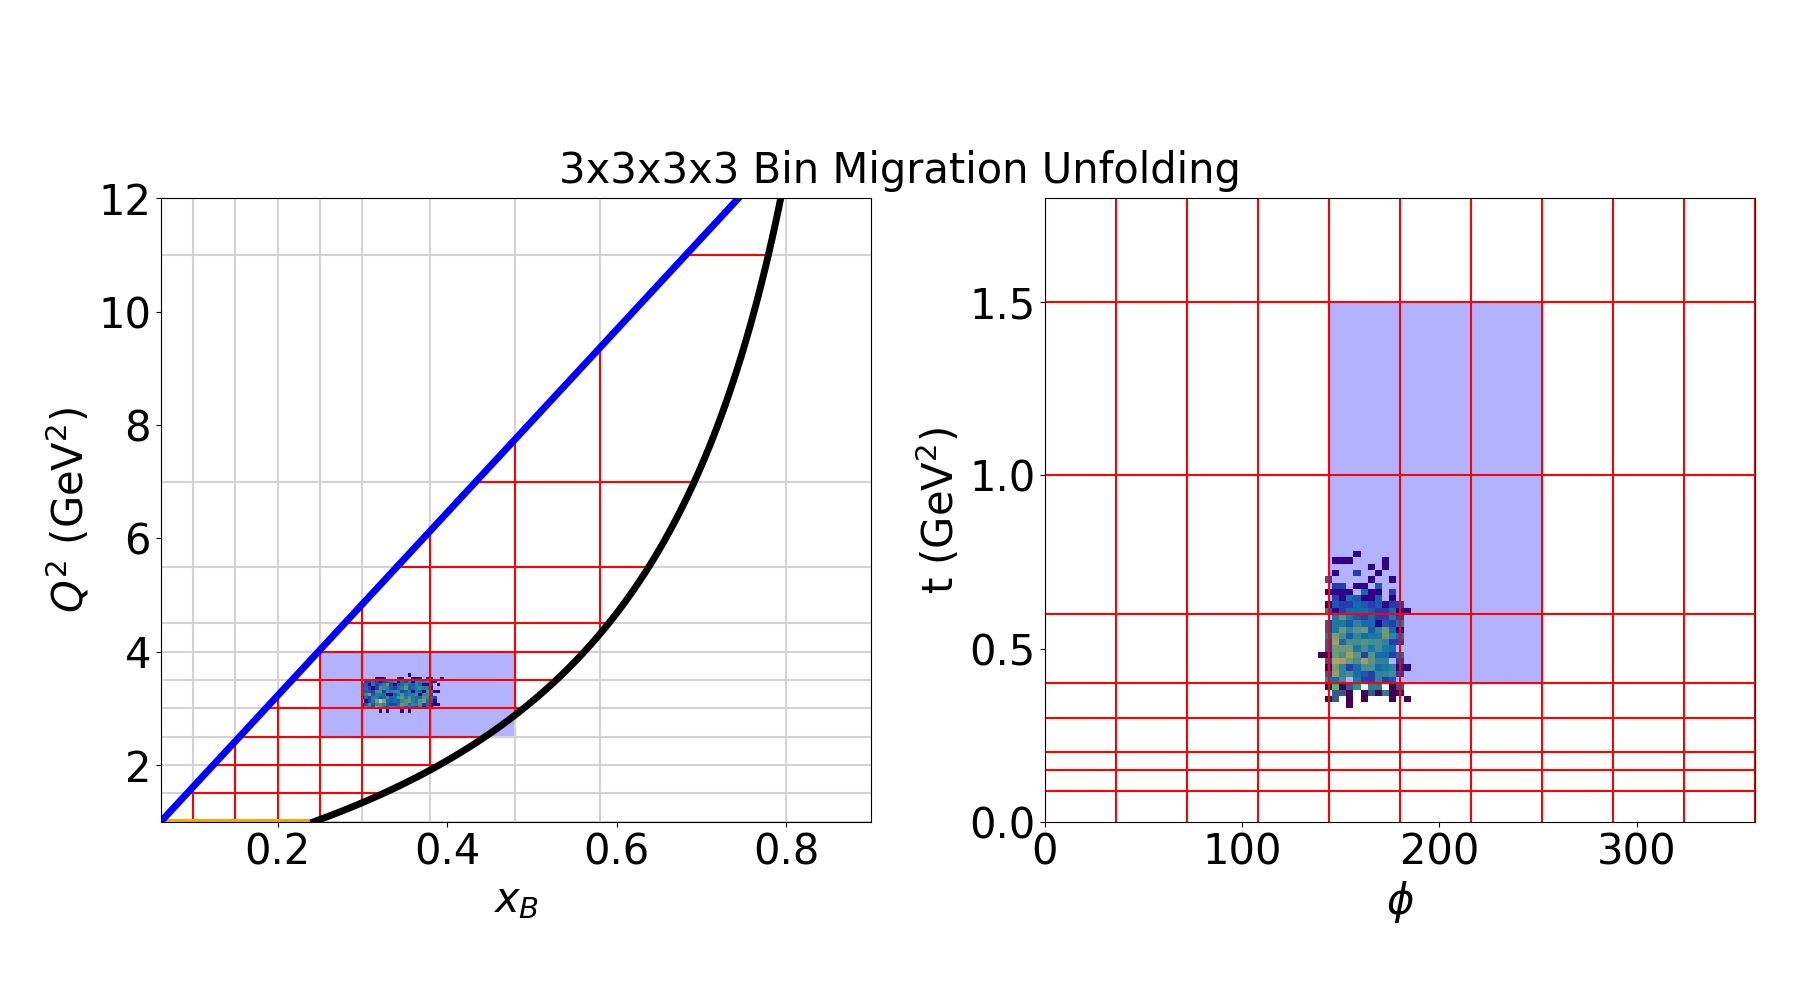
\includegraphics[trim={22.5cm 0 0 5cm},clip,width=0.3\textwidth]{Chapters/Ch5-Further/0_IBU/pics/kerneling/bin_migration_1_1_0_0.png}}\\
    \caption{Caption for your 3x3 grid of figures}
    \label{fig:test}
    \end{figure}
    
\clearpage
\section{Unfolding Matrix Results}

    We processed on the whole dataset

    \iffalse
    \begin{figure}[ht]
        \centering
        \subfloat[]{
            \begin{tikzpicture}
                \node[anchor=south west,inner sep=0] (image) at (0,0) {
                    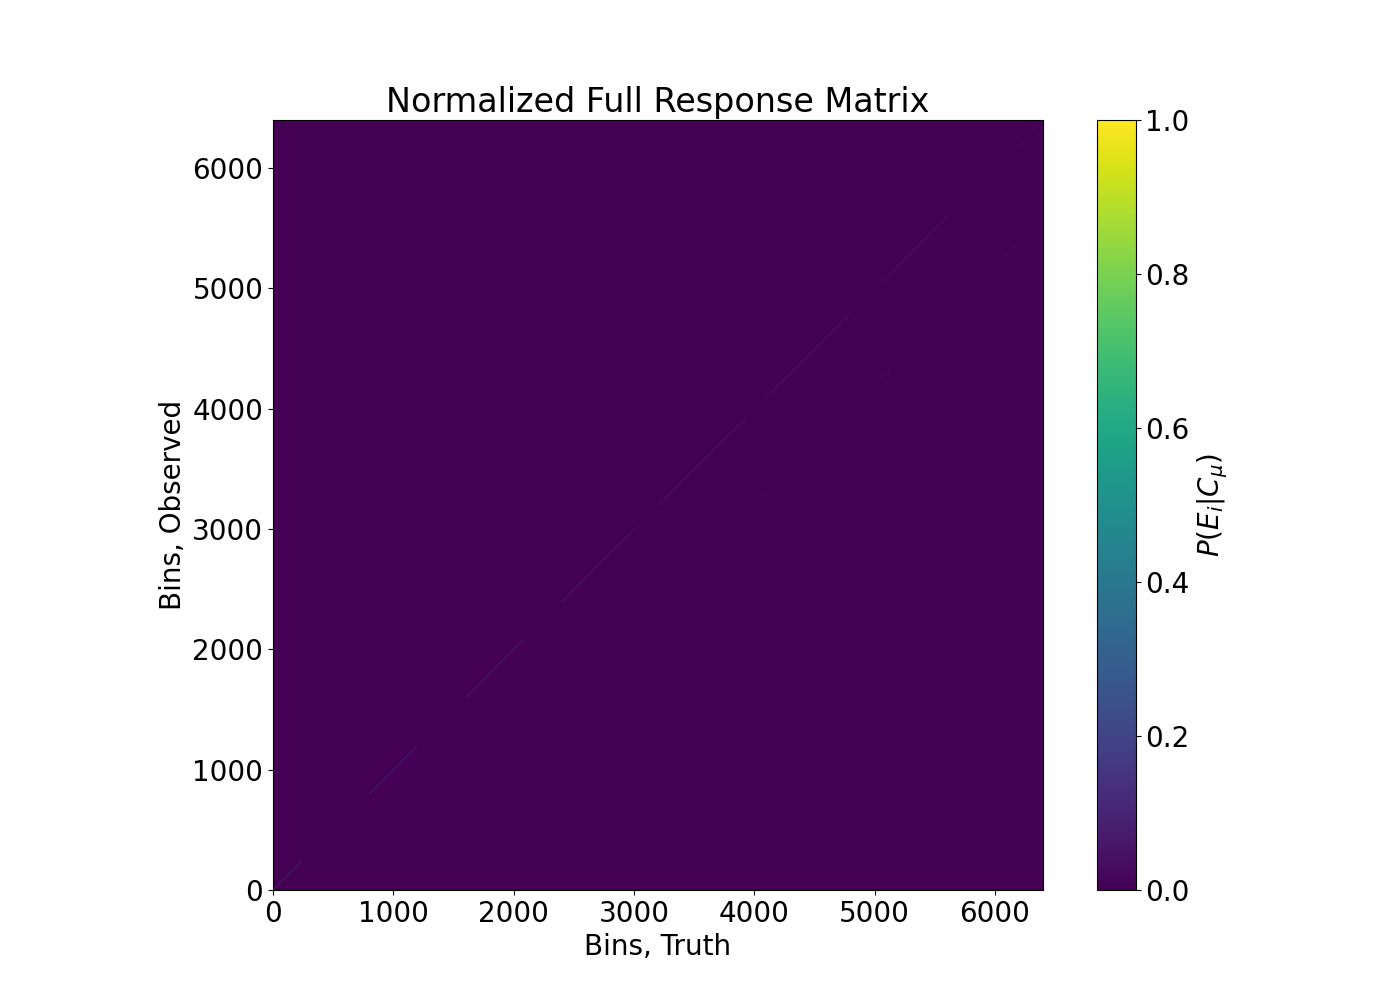
\includegraphics[trim={0 0 0 0},clip,width=0.45\textwidth]{Chapters/Ch5-Further/0_IBU/pics/4D_all_bins_normalized_full_response_matrix.png}
                };
                \begin{scope}[x={(image.south east)},y={(image.north west)}]
                    \draw[red,ultra thick] (0.43,0.45) rectangle ++(0.1,0.1.5); %Change the values as per your need
                \end{scope}
            \end{tikzpicture}
            \label{fig:ibu1}
        }
        \hfill
        \subfloat[]{
            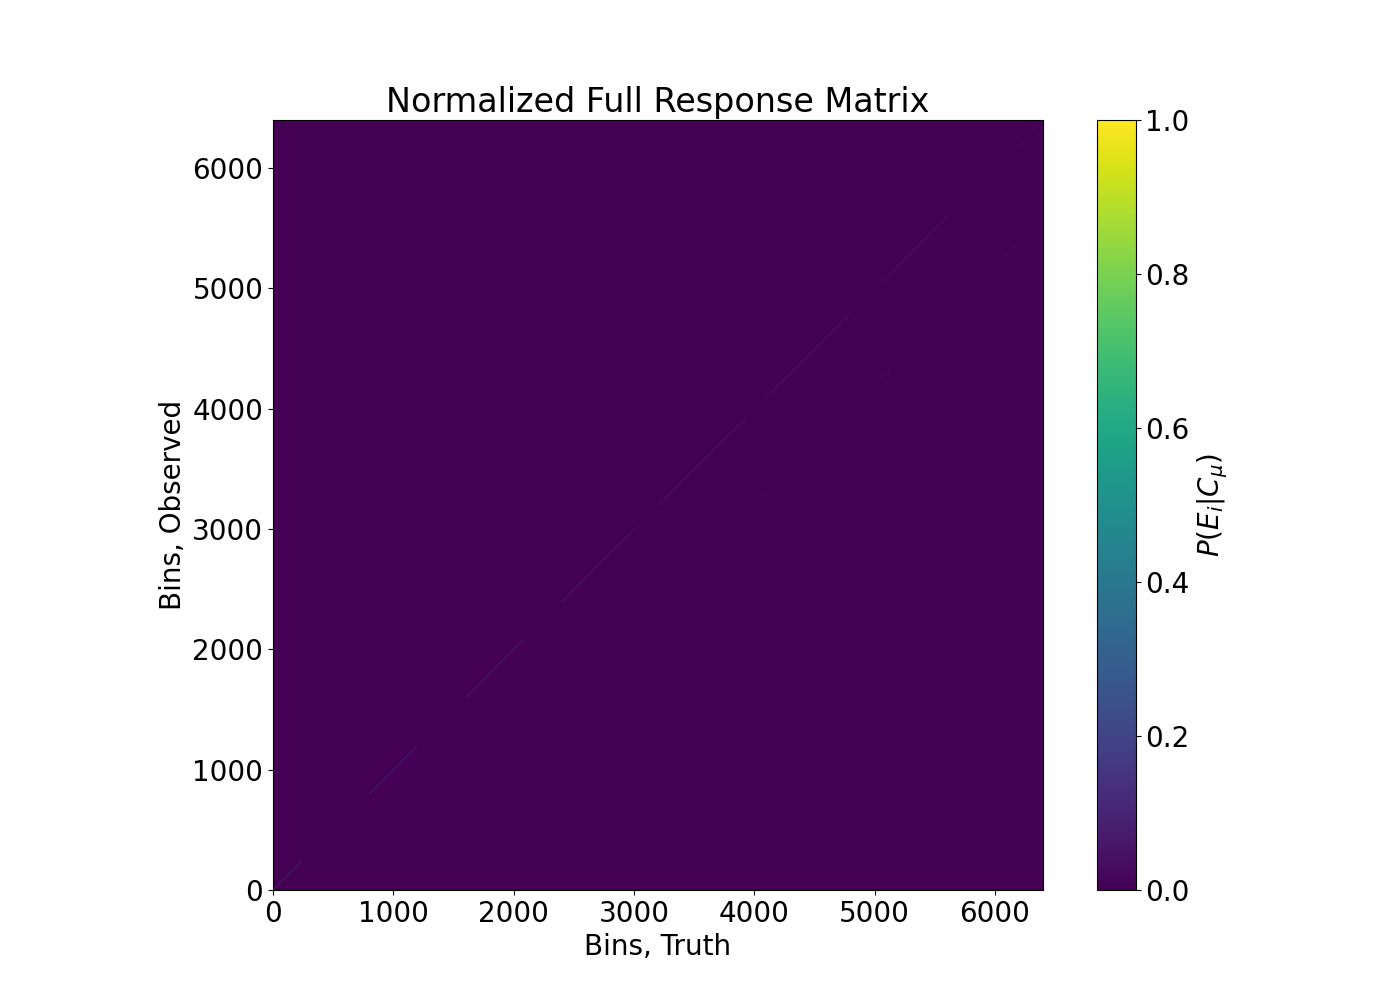
\includegraphics[trim={16cm 12cm 17cm 11cm},clip,width=0.4\textwidth]{Chapters/Ch5-Further/0_IBU/pics/4D_all_bins_normalized_full_response_matrix.png}
            \label{fig:ibu2}
        }
        \caption{Caption for both figures}
        \label{fig:ibu}
    \end{figure}
    \fi


    
    \begin{figure}[ht]
    \centering
    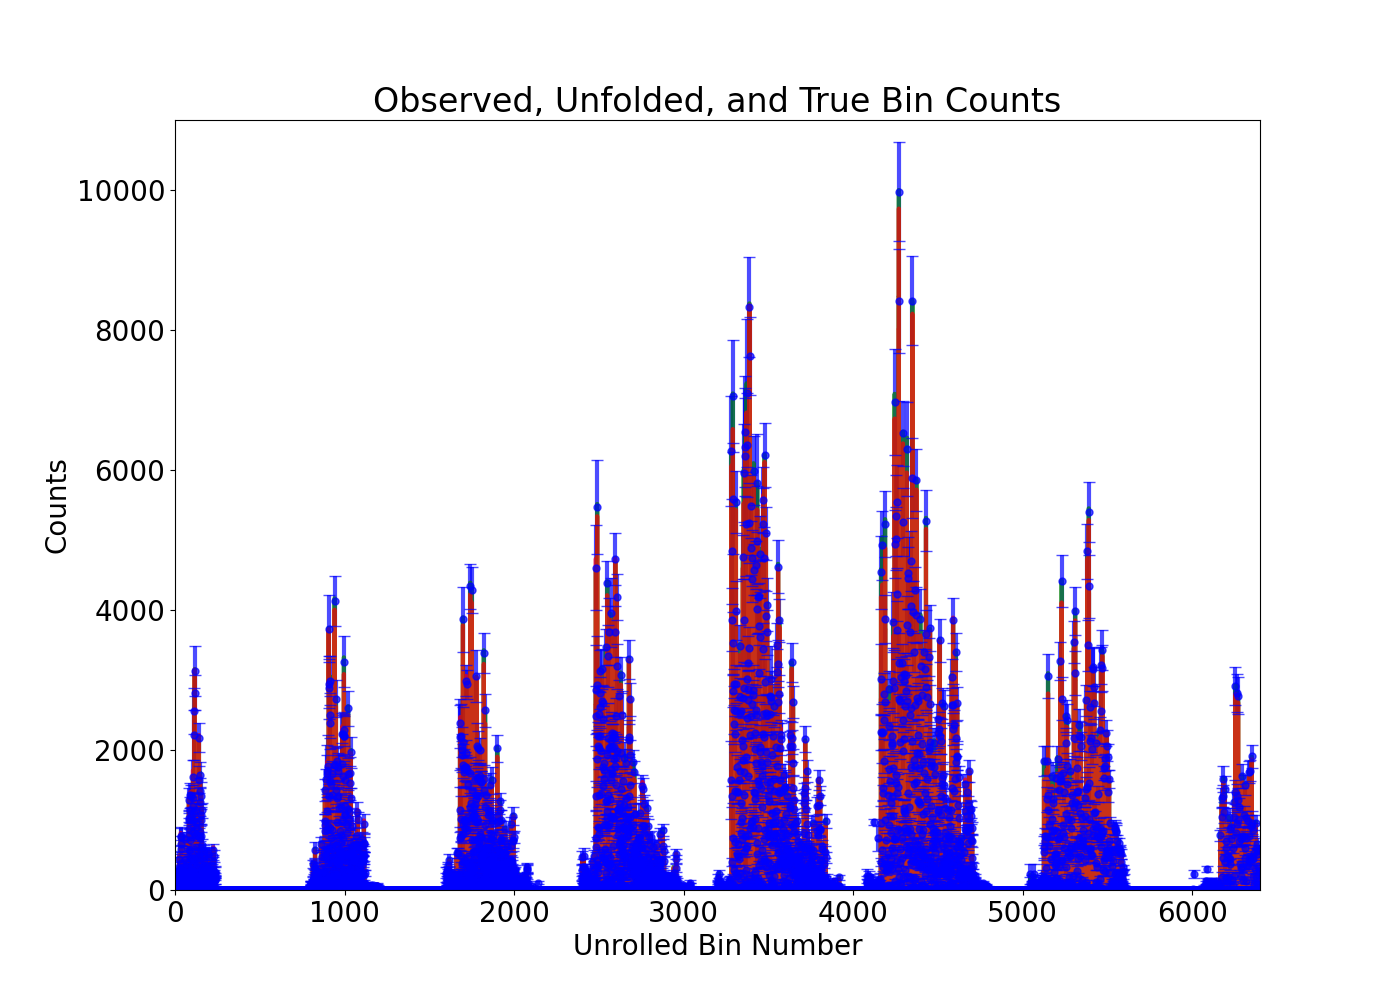
\includegraphics[trim={0 0 0 0},clip,width=\textwidth]{Chapters/Ch5-Further/0_IBU/pics/complete/observed_unfolded_and_true_bin_counts.png}
    \caption[words]{words}
    \label{fig:ibu2}
    \end{figure}
    
    \begin{figure}[ht]
    \centering
    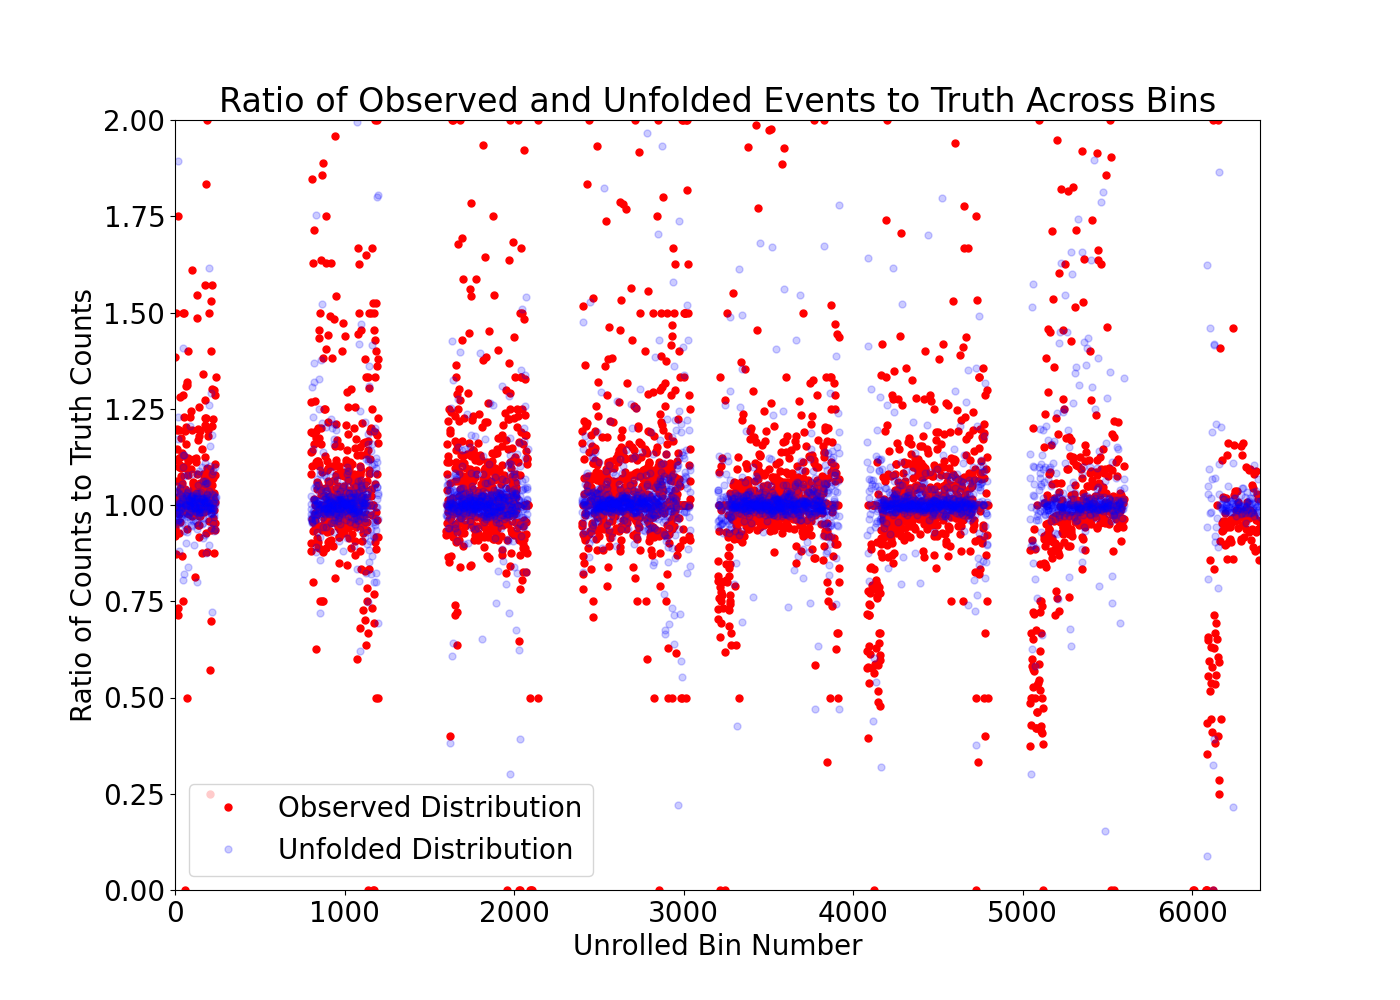
\includegraphics[trim={0 0 0 0},clip,width=\textwidth]{Chapters/Ch5-Further/0_IBU/pics/complete/ratio_of_observed_and_unfolded_events_to_truth_across_bins.png}
    \caption[words]{words}
    \label{fig:ibu3}
    \end{figure}

    
    \begin{figure}[ht]
    \centering
    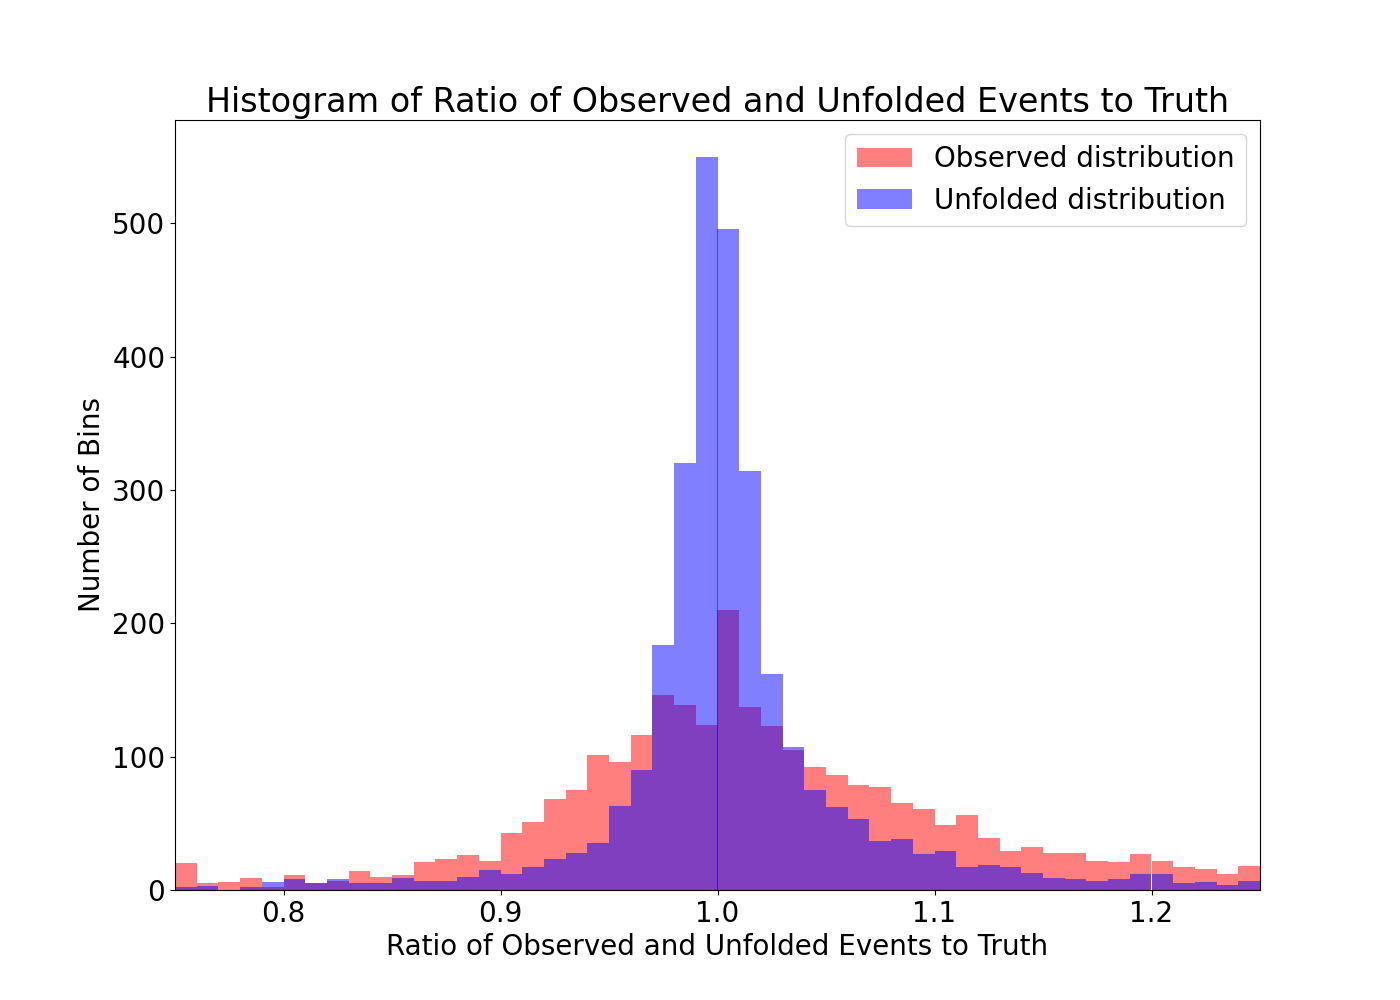
\includegraphics[trim={0 0 0 0},clip,width=\textwidth]{Chapters/Ch5-Further/0_IBU/pics/complete/histogram_of_ratio_of_observed_and_unfolded_events_to_truth.png}
    \caption[words]{words}
    \label{fig:ibu1}
    \end{figure}
    
\clearpage

\section{Unfolding Effect on Cross Section Values}

 TO DO: COMPARE BIN BY BIN and make histogram of comparisons